\chapter{Computational Creativity and Task Conditioning}\label{ch-task-conditioning}
\section{Introduction}

The task in this dissertation is defined as the input a solver consumes in kinematic synthesis. For motion generation, the task is a set of poses\footnote{combination of positon and orientation} that describe the intended motion. In the case of path generation, the task is a set of points describing the path. Since the task is devoid of knowledge about the outcome of solvers, there is no way of knowing if the task is ill-posed. The task conditioning is the process in which the task is modified to make it more conducive for the solvers. In addition, the task conditioning can also include informed modification for satisfying the desired context. This chapter presents the details on how such informed modifications are achieved using a data-driven strategy. Section~\ref{sec_task_conditioning_overview} presents the details of the process. Section ~\ref{sec_data_prep} presents data preparation and representation for motion and path tasks. Section~\ref{sec_task_conditioning_image} presents examples of feasibility conditioning of tasks. Section~\ref{sec_context} presents how a context function can be learned in a data-driven way.    
\section{Task Conditioning Overview}\label{sec_task_conditioning_overview}
To such modifications, it is imperative to possess knowledge about the properties of the task. This knowledge is expressed as a prior probability distribution, often simply called the \emph{prior}. This work uses Variational Auto-Encoders (VAE) to learn this \emph{prior} by learning from a set of real coupler trajectories of randomly constructed linkages. Thus, the recognition model of a VAE is trained to compute a maximum a posterior probability (MAP) estimate of latent features for the given input given by,
\begin{eqnarray}
  \mu, \sigma = Q(X_{task}), \\
  z \sim \mathcal{N}(\mu, \sigma).
\end{eqnarray}
Here, $z$ is a sample from the recognized latent distribution. This distribution can be thought of as a distribution of recognized properties of coupler curves that were observed in the task by recognition model.  

Then, the generative model of VAE generates few samples from approximate marginal likelihood distribution of recognized latent features given by,
\begin{equation}
  \hat{X} \sim G(\mathcal{N}(\mu, \sigma)).
\end{equation}
Here, $\hat{X}$ is a sample from a distribution computed by approximate marginal inference for a given input task $X_{task}$ and is given by,
\begin{equation}
  \hat{X} \sim pr(X|X_{task}) \approx \int pr(X|z)pr(z|X_{task})dz.
\end{equation}
Intuitively, it represents a modified task after applying a \emph{prior} function which was learned in a data-driven way.
VAE computes a distribution $(pr(\hat{X}|X)$ of such modified tasks, which are then inputted to synthesis solvers. These modified tasks are termed as \emph{Variational Inputs}. 


\section{Representation of Tasks}\label{sec_data_prep}
This section presents the details of the normalization and representation of tasks in various formats. In this work, we showcase the conditioning of tasks for path and motion generation problems.

First, consider a database of coupler paths formed by planar linkages. Each coupler path is an ordered collection of $m$ points sampled uniformly throughout the entire rotation of the crank, where each point has $x$ and $y$ coordinate.
Thus, each coupler curve \ac{x_path_vector} is $\{x_j, y_j\}_{j=1}^{m}$ and each coupler motion \ac{x_motion_vector} is $\{x_j, y_j, \theta_j\}_{j=1}^{m}$ for motion data. Both of the task representations are first normalized before feeding to \ac{vae}.

\subsection{Data Normalization}

First, each coupler trajectory is normalized with respect to scale and position.
This is done by subtracting the means $(\bar{x}, \bar{y})$ and dividing by the root mean squared variance in Cartesian $X$- and $Y$-directions.
Next, the trajectory is rotated such that its principal component axes are aligned with the coordinate axes.
The principal component axes are the eigenvectors of the covariance matrix of a point cloud data that defines the trajectory.
The covariance matrix $C$ of a point cloud of $m$ 2D points $\{x_j, y_j\}_{j=1}^{m}$ is given by,
\begin{eqnarray}
  C = \left[
\begin{array}{cc}
  C_{xx}  & C_{xy}  \\
  C_{yx}  & C_{yy}
\end{array}
\right],\\
C_{xx} = \frac {1}{m} \sum_{i=1}^{m}(x_i - \bar{x})(x_i - \bar{x}) ,\\
C_{yy} = \frac {1}{m} \sum_{i=1}^{m}(y_i - \bar{y})(y_i - \bar{y}) ,\\
C_{xy} = C_{yx} = \frac {1}{m} \sum_{i=1}^{m}(x_i - \bar{x})(y_i - \bar{y}).
\end{eqnarray}

Figure~\ref{fig_curve_normalization} depicts the normalization procedure for two couple paths.

\begin{figure}
\centering
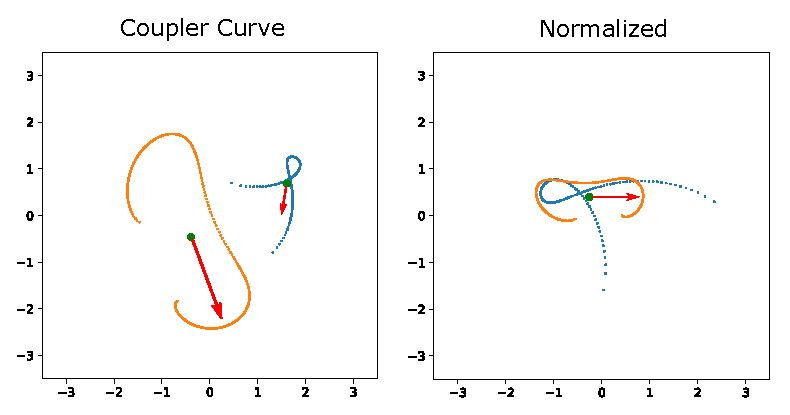
\includegraphics[width=0.7\textwidth]{idetc-20/figure/fig_curve_normalization.eps}
  \caption{Each curve is normalized for position, scale and orientation.}
\label{fig_curve_normalization}
\end{figure}


Another common approach is to treat this sequence of points $\{x_j, y_j\}_{j=1}^{m}$ as a one dimensional temporal signal with parameter $t$ given by,  
\begin{equation*}
    \textrm{CC} = \{x(t), y(t)\}
\end{equation*}

This formulation allows for applying various signal processing techniques like Fourier Analysis. While this type of modeling has many advantages which are evident by the success in path generation~\cite{wu2011},\cite{ullah1997}, it fails to capture spatial correlations that are not implicit in temporal correlations.

\subsection{Representing Task as an Image}\label{sec_image_representation}

The proposed image-based representation allows us to capture those correlations in exchange for losing temporal correlations between the input sequences.
However, it can be argued that the ordering is embedded in the spatial distribution of pixels since unlike typical computer vision applications, such as facial recognition, which have a true 2D set of pixels for images, a curve is fundamentally a one-dimensional entity only. In addition, if the task does not need a specific ordering of points, the image-based approach allows for capturing all possible input orders in a unified way. An image represents a probabilistic coupler curve, where the intensity of a pixel represents the likelihood of containing a coupler curve point. First, each coupler curve is normalized with respect to scale, position, and orientation.


The normalized planar curve is now discretized into a 2D image. The two-dimensional Cartesian space is linearly discretized into $S-1$ partitions along each axis, where $S$ corresponds to a side of the image.
The partitions along x-axis is done as follows:
$x$ coordinates that lie between $-\infty$ to $-x_{lim}$ are binned into a the first partition. The next partition includes $x$ ranging from $(-x_{lim}, -x_{lim} + x_{step}]$, and so on up to the last partition $(X_{lim}, +\infty)$. Here, $x_{lim}$ and $x_{step}$ are discretization parameters, which control the range and resolution respectively. Figure~\ref{fig_curve_discretization} depicts the discretization of a normalized curve. It can be noted that the extreme coordinates play an important role in deciding resolution and range of pixels. 


\begin{figure}
\centering
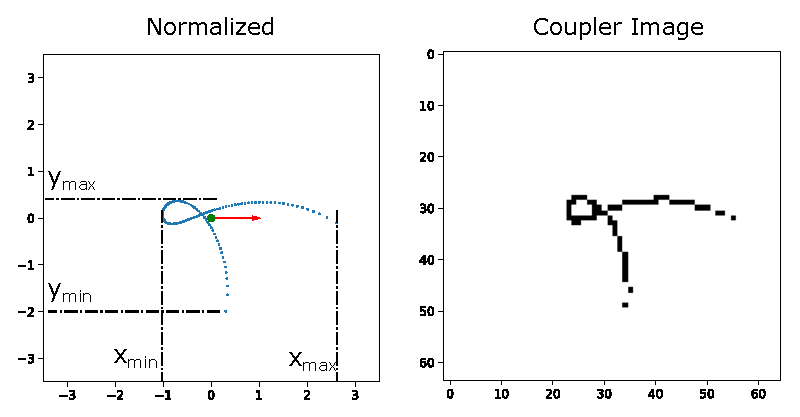
\includegraphics[width=270pt]{idetc-20/figure/fig_curve_discretization.eps}
  \caption{The extreme coordinates ($x_{min}, x_{max}, y_{min}, y_{max}$) of a normalized coupler curve are shown. If a point lies in Cartesian span of pixel, it is given 1.0 probability.}
\label{fig_curve_discretization}
\end{figure}


\begin{figure}
\centering
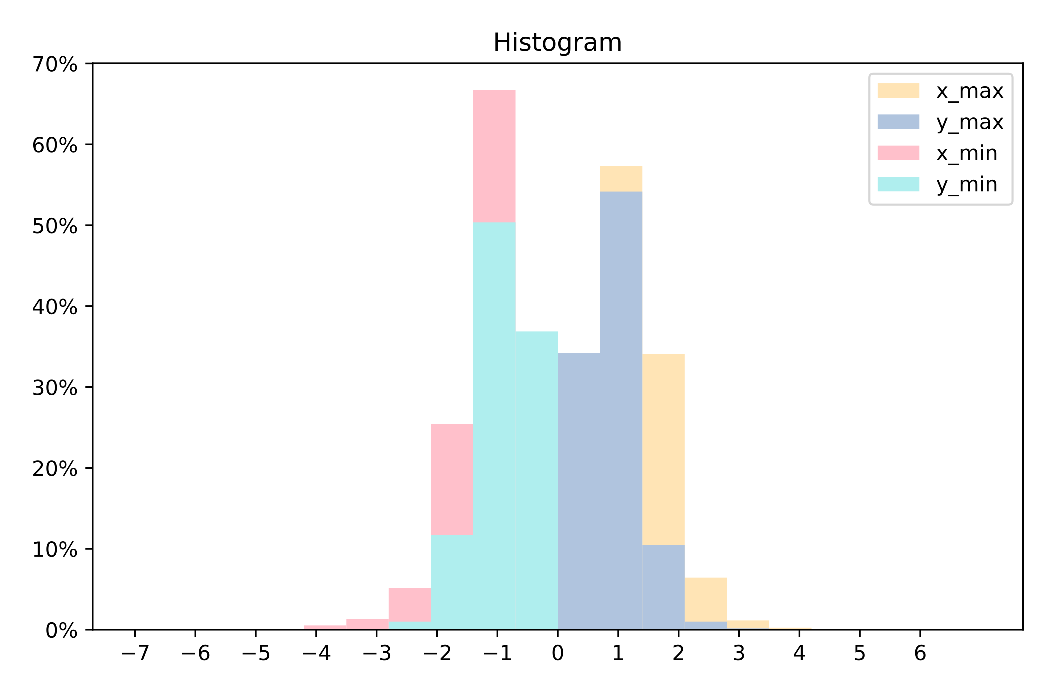
\includegraphics[width=300pt]{idetc-20/figure/fig_histogram.eps}
  \caption{A histogram of extreme coordinates ($x_{min}, x_{max}, y_{min}, y_{max}$) of coupler curves. It can be seen that less than $1\%$ of the normalized coupler curves have a point with an absolute coordinate larger than 3.5 units.}
\label{fig_histogram}
\end{figure}




To estimate $x_{lim}$, a statistical study is conducted on a dataset of 6,818 linkages comprising of four-bar (2,188), Stephenson I (2,754) and Stephenson III (1,876) six-bar linkages. The coupler curve for each linkage is stored as a sequence of points sampled per one-degree change in the crank angle. The number of points in coupler curves is different for different mechanisms. Figure~\ref{fig_histogram} shows the histogram of extreme coordinates corresponding to the normalized coupler curves from the database. It can be seen that more than $99\%$ of linkages are contained by a square with a side 7 and center at the origin. Thus, $x_{lim}$ is set as $7/2 = 3.5$. 
For an image with ($S\times S$) pixels, $x_{step}$ is given by,
\begin{equation*}
   x_{step} = \frac{2x_{lim}}{S - 1}.
\end{equation*}
Here, each pixel of an image represents a probability of containing at least one point of the coupler curve.
In this work, we choose $S = 64$, which provides sufficient resolution to capture the variation in coupler curves. 
Figure~\ref{fig_curve_discretization} depicts the discretization of a normalized coupler curve into an image.
It should be noted that the discretization process causes some loss of information. However, in many cases, the input is inherently vague. Thus, it acts as a buffer and prevents the further process from over-emphasizing the numerical precision. One can also notice that image-based representation removes the order of points in the curve. However, it grants spatial correlations between neighboring points, which helps in capturing interesting spatial patterns.


\section{VAE Training}

\begin{figure}
\centering
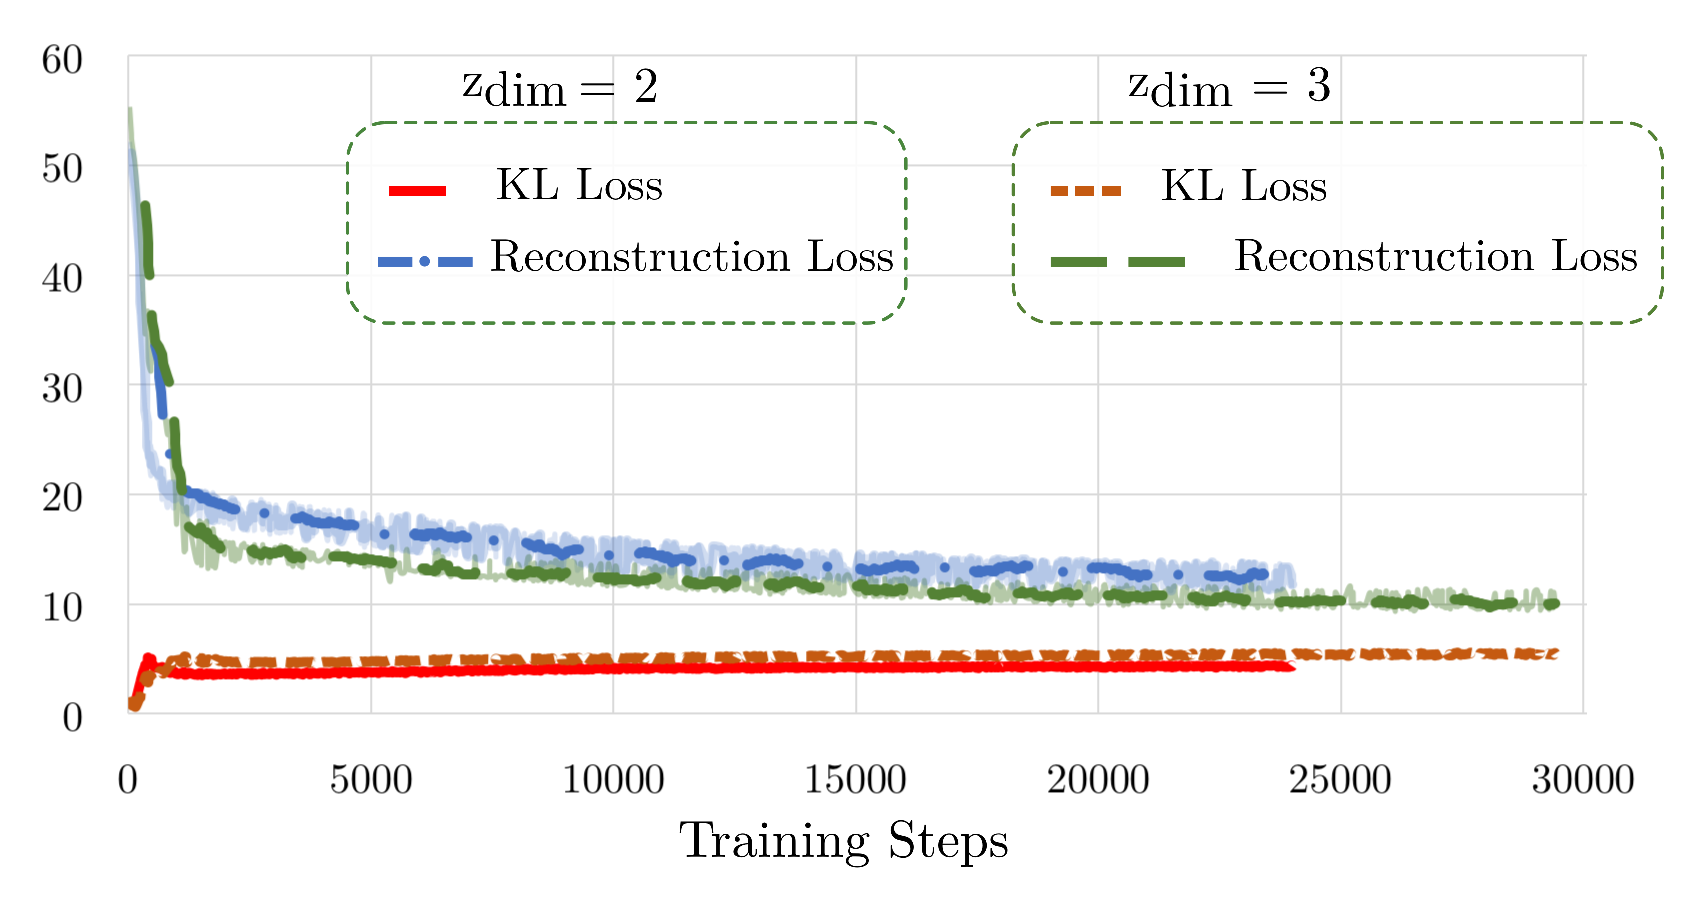
\includegraphics[width=240pt]{jmd-19/figure/fig_vae_train_loss.eps}
  \caption{Reconstruction and KL Divergence losses for two architectures with z dimension 2 and 3. It can be seen that higher z-dimension enables capturing more variation in the database, which results in lower reconstruction losses.}
\label{fig_vae_training_loss}
\end{figure}


\begin{figure*}[t]
\centering
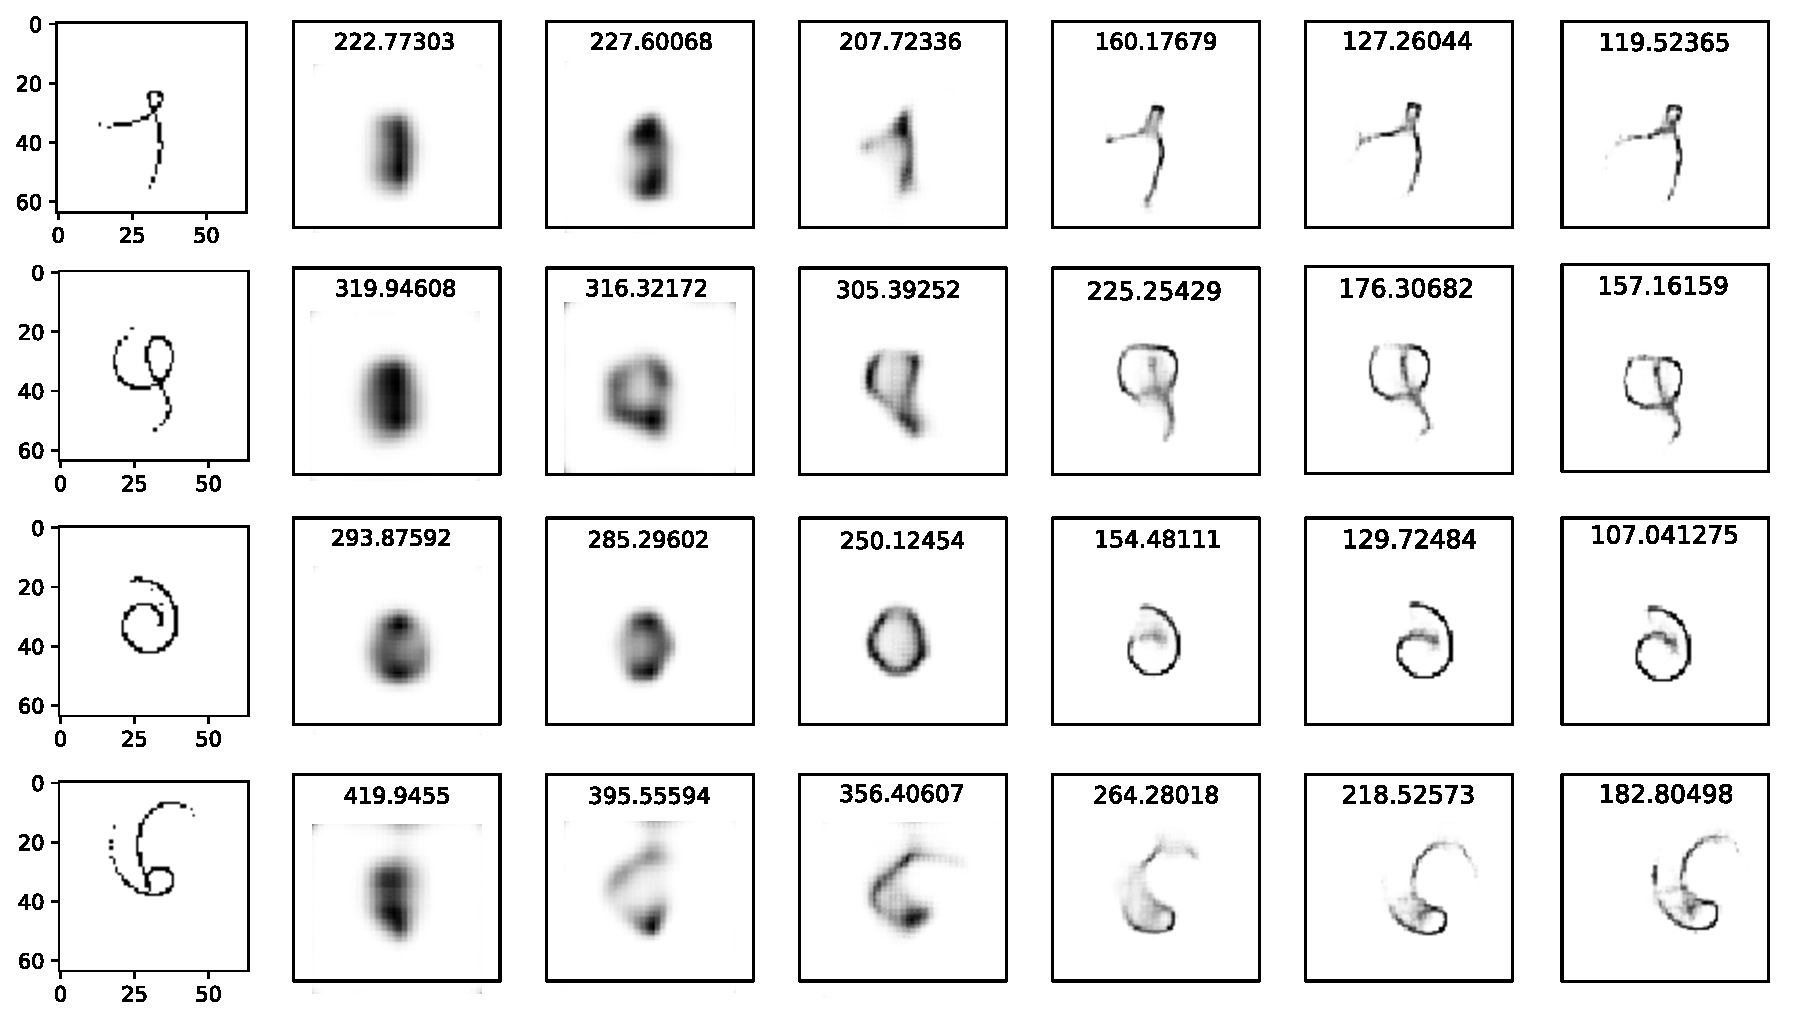
\includegraphics[width=0.75\textwidth]{idetc-20/figure/training_testing.eps}
  \caption{The training progress is reflected in the reconstruction quality of test coupler curve images. The corresponding variational lower bound $L_{ElBo}^{X^i}$ is displayed above each reconstructed image. It can be seen that the probability assignment by VAE for each pixel improves over the training.}
\label{fig_training_reconstructions}
\end{figure*}

Various datasets of linkages are used to train various architectures of VAE with varying numbers of latent dimensional size. A new linkage is added to the dataset if it is sufficiently dissimilar from all the linkages previously added to the dataset.
Here, the measure of dissimilarity between two linkages is given by a sum of $L2$ norms between the normalized trajectories traced by all moving points of two linkages.
Table ~\ref{tab_dataset} presents the details on various datasets used for training.

Figure~\ref{fig_vae_training_loss} depicts training losses for two such architectures with latent dimension (i.e., the dimension of $z$ vector) 2 and 3.
As we can see in Fig.~\ref{fig_vae_training_loss}, the model with a 3-dimensional $z$ vector space achieves lower reconstruction error with slightly higher KL divergence loss.
This result is expected because with an increase in latent size, the room to capture variation in the data increases.
However, the increase in the latent dimension also increases the complexity in visualization, interpretation, and manipulation of latent attributes in recognition tasks.
It is interesting to notice that the two losses somewhat compete with each other in the training process.
The reconstruction loss pushes the model to capture the diversity in the dataset, by forcing the generator to be able to reconstruct every type of data in the dataset. Whereas, KL divergence forces the latent space to occupy a restrictive distribution and thereby demanding coherence in the generation.


Figure~\ref{fig_training_reconstructions} shows improvement in reconstructions of coupler image samples from the test set as the training progresses. It can be seen that the pixels with a higher probability of containing a coupler point are assigned a higher probability and vice versa. 
Once the network is trained sufficiently, the encoder learns to capture spatial correlations and returns a probability distribution in latent feature space. Each sample from this distribution has a high probability of being a valid coupler image. 
This feature is used to obtain feasible representations of raw input and is demonstrated in Section~\ref{sec_task_conditioning_image}. 


\begin{table}
  \caption{Datasets used for Training VAE}
\centering
\label{tab_dataset}
\begin{tabular}{cc}
\hline
  Data Type & Size \\
\hline
  Four-bar Linkage (Grashof Only) & 480 \\
  Four-bar Linkages & 2188 \\
  Slider-Crank Linkages (Grashof Only) & 466 \\
  Six-bar Stephenson IIIa Linkage (Grashof Only) & 937 \\
  Six-bar Stephenson IIIa Linkage & 3902 \\
\end{tabular}
\end{table}


\begin{figure*}
\centering
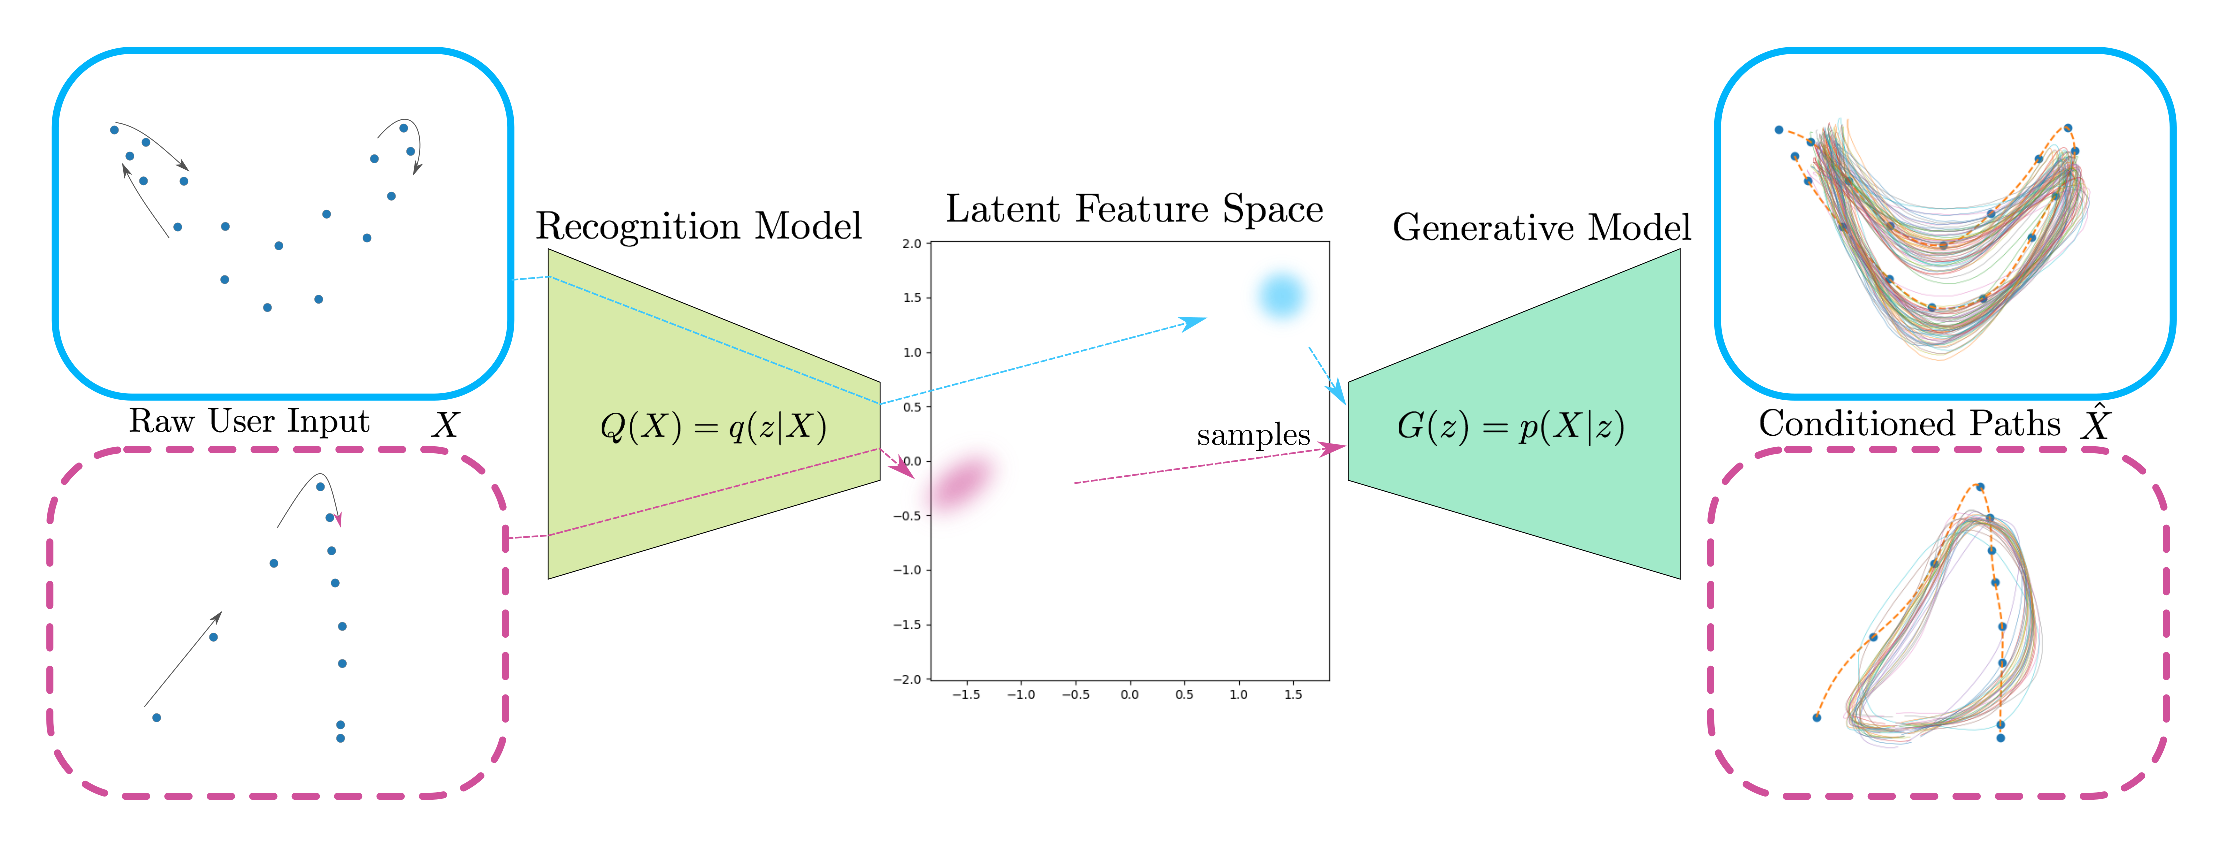
\includegraphics[width=\textwidth]{jmd-19/figure/fig_recognition_model.eps}
  \caption{The raw user input $X$ is passed through a recognition network, which captures the salient information in the form of multivariate distribution of latent features. Random samples from this distribution are fed to the generator to generate paths with a high likelihood of producing good solutions. Moreover, users can manipulate the sample location in latent space, which gives them a low-dimensional and higher level of control on modifying the shape of the path.}
\label{interactive_recognition}
\end{figure*}

\section{Recognition and Generation of Coupler Trajectories}\label{sec_recogn_cp}
For training or inference, each data point \ac{x_path_vector} is passed through a recognition model that computes the parameters for multivariate Gaussian distribution of latent vector.
In inference, the aim is to recognize the salient features of the input point cloud.
To showcase the inference functionality, let us consider two-point sequences that are obtained by manually drawing points on an interface.
Each of the sequences represents an approximate target path.
Now we would like to infer their salient features and generate plausible coupler paths having similar salient features.
We take a trained VAE with two-dimensional $z_{\text{path vector}}$ vector trained on closed coupler paths (VAE-z2-path).
The two-point sequences, one at a time is passed through a recognition network, which predicts a 2-D Gaussian distribution of latent features for each of the input as shown in Fig.~\ref{interactive_recognition}.
Now for each case, random samples drawn from the distribution are passed to the generator network of the VAE, it generates the samples with closed paths that resemble the original input path as shown in Fig.~\ref{interactive_recognition}.

\section{Interactive Shape Modification with VAE}
Let us assume a scenario where the user needs to specify a closed-loop target path.
Since the synthesis of linkages is chaotic, it is always fruitful to condition the inputs such that the probability of finding good linkages is maximized.
Moreover, it is desirable to have a higher level of control on the overall shape of the target path.
We use VAE to accomplish both of the above tasks.
First raw user input \ac{x_path_vector} is passed through recognition model as shown in Fig~\ref{interactive_recognition}.
The recognition model captures the shape user intends to draw and returns it in the form latent feature distribution $q(z|X)$ as shown in Fig.~\ref{interactive_recognition}.
The VAE generator takes a sample feature vector $z_s$ from $q(z|X)$ and generates a path $\hat{X}$.
It should be noted that $\hat{X}$ is a sample from the distribution $p(X|z)$ and has more probability of being a path drawn from a four-bar.
As we can see in Fig~\ref{interactive_recognition}, generated paths follow the user-defined points, but also resemble paths generated by Grashof four-bar linkages.
Moreover, the user can select or modify the $z_s$ interactively based on the variation of its corresponding generated path.
Hence, the user has a higher level control on the shape of the path which improves the experience rather than modifying the input path point by point.
This can be achieved by creating a user interface where the user can see the effects of changing feature vector $z$ in all possible directions.
Figure~\ref{vae_fb_random_samples} presents samples created by the generator for different latent vectors.
Here, the user can visualize where the given curve lies, and change its shape by moving across the plane in 2-D.
This approach is amenable if the dimensionality of feature vector $z$ is kept below $4$].
\begin{figure}
\centering
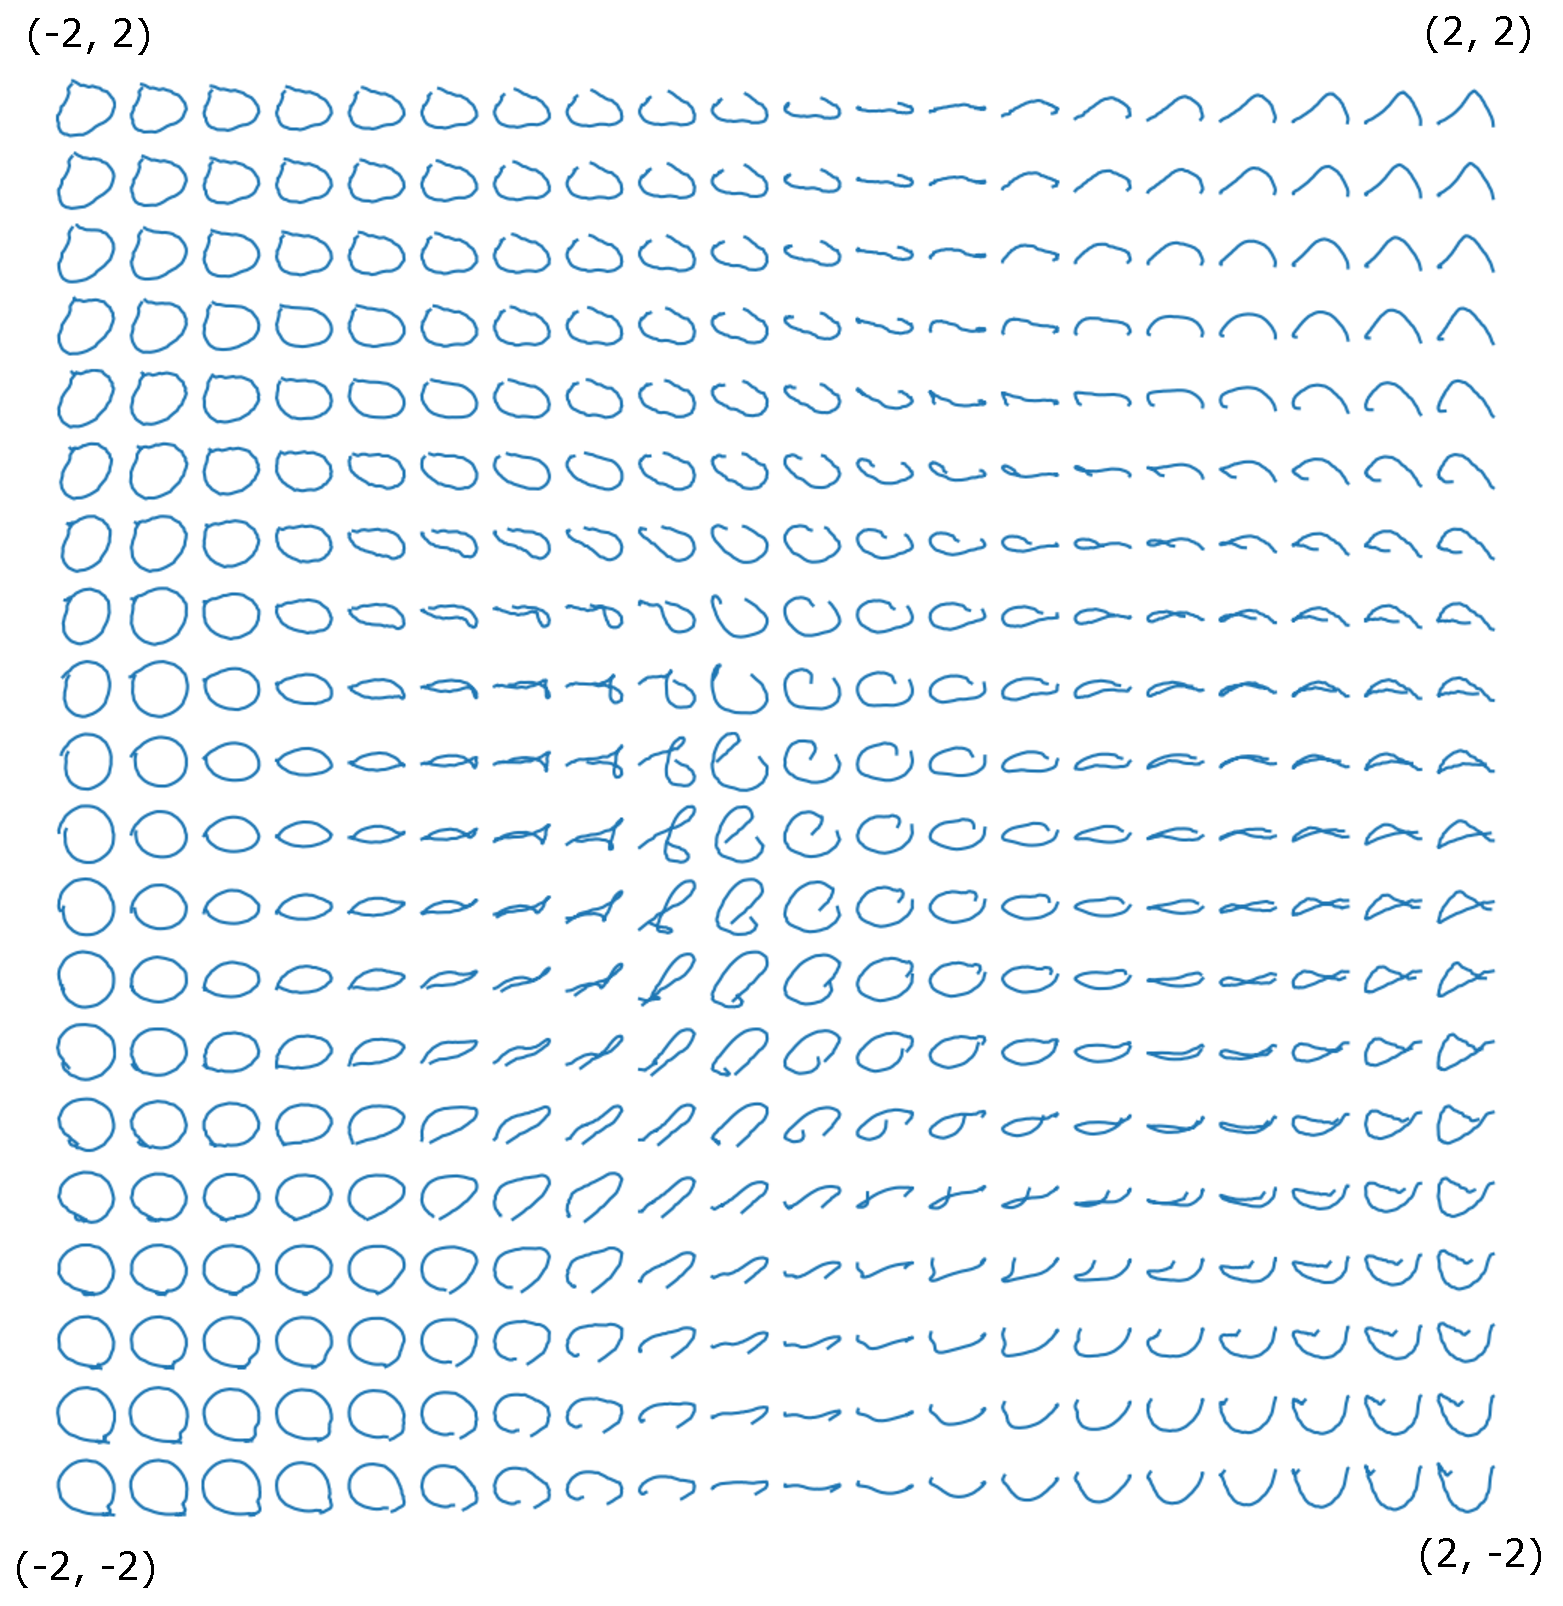
\includegraphics[width=240pt]{jmd-19/figure/path_embedding_with_grid.eps}
  \caption{Samples generated from a generator from a two-dimensional latent vector which is a vertex in the two-dimensional uniform grid with limits shown in corners. It can be seen that samples generated from neighboring vertices are highly correlated, which gives away the indication that recognition network learns the salient information about the shape of coupler curves.}
\label{vae_fb_random_samples}
\end{figure}


\subsection{Type Synthesis via Recognition}
Several VAEs with different architectures are trained on the dataset that comprises of coupler paths, motions from four-bars, slider-cranks and Stephenson type six-bars.
Since the linkages above have a different topology, their coupler motions should possess some features that are affected by it.
Figure~\ref{fig_classifier} depicts 2-D embedding of closed coupler paths from Four-Bar (all revolute joints), Slider-Crank and Stephenson six-bar mechanisms.
It can be clearly seen that six-bar coupler curves cover a wider variety in shape compared to four-bar linkages.
Variety covered by slider-crank linkages is the lowest and is mostly overlapped by a four-bar linkage.
The reasoning behind this observation can be given by the fact the slider-crank linkages are a special case of 4R linkages when the length of the rocker link and its fixed pivot approach infinity.
A classifier trained on such data can predict the probabilities of a given task being fulfilled by the corresponding linkage type.
\begin{figure}
\centering
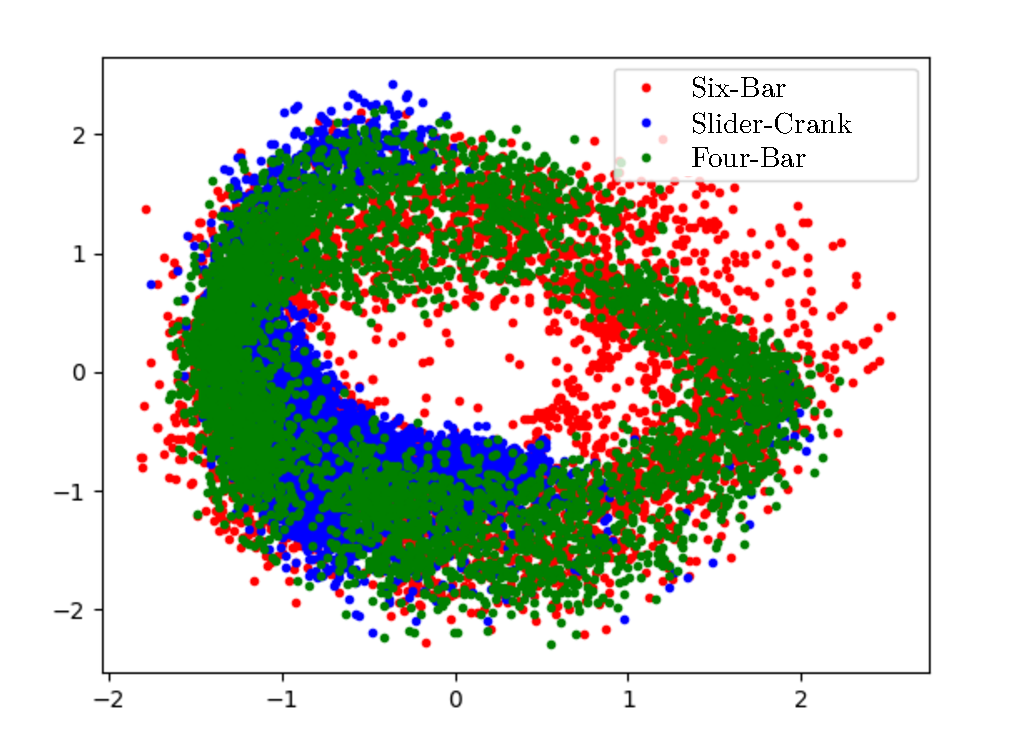
\includegraphics[width=240pt]{jmd-19/figure/fig_classifier.eps}
  \caption{Visualization of 2-D feature embedding obtained by training a VAE on closed coupler paths of various planar linkages. The variety in features by means of spread over the space directly relates to the variety in the shape of respective linkage type.}
\label{fig_classifier}
\end{figure}


\subsection{Example User-ML Interaction}\label{example_interaction}
In this section, we showcase the application of VAE to solve a path generation problem using a motion generation problem solver.
As we have stated earlier, the ML Intermediary can take crude input from the user and provide all the necessary information required by available solver with computational subtleties.
These tasks require VAE to capture primitive information provided by raw user input and generate a set of plausible coupler motions.
It is important to note that since the orientation information required by the motion generation solver is not provided by the user, it should be guessed by the ML Intermediary.
This is done by using a C-VAE that is trained to generate coupler motions \ac{x_motion_vector} data given its path \ac{x_path_vector}.
The architecture and training scheme for the C-VAE follows the discussion presented in Chapter~\ref{condi_vae}.
We use our computational methods~\cite{generalfitting-JCISE},\cite{shrinathpurwar2017} for solving the motion generation problem in real-time.
The solutions returned by the solver are fed to the linkage recognition model of a VAE trained on entire four-bar linkages.
This linkage recognition model computes a compact feature representation of each linkage on which we apply the K-means\cite{lloyd1982kmeans} clustering algorithm.
The details of linkage recognition and clustering are presented in section~\ref{subsec_vae_for_ln}.
It should be noted that the feature distributions of linkages produced by a recognition model are in ten-dimensional space.
Thus, the depiction of the latent distribution of linkages and following clusters as shown in Fig.~\ref{fig_user_interaction} are only for illustration purposes.
The cluster centers are distinct solution concepts. Figure~\ref{fig_user_interaction} depicts the entire procedure from start to finish.
The solutions obtained using the proposed approach yields diverse mechanisms with various linkage topologies.
To juxtapose our approach with classical approaches, Fig.~\ref{fig_user_interaction} also depicts the result obtained using a classical path synthesis method~\cite{sharma2019optimal} based on Fourier Descriptors.
It can be seen that the classical result is similar to one of the concept solutions obtained using variational synthesis.

\begin{figure*}
\centering
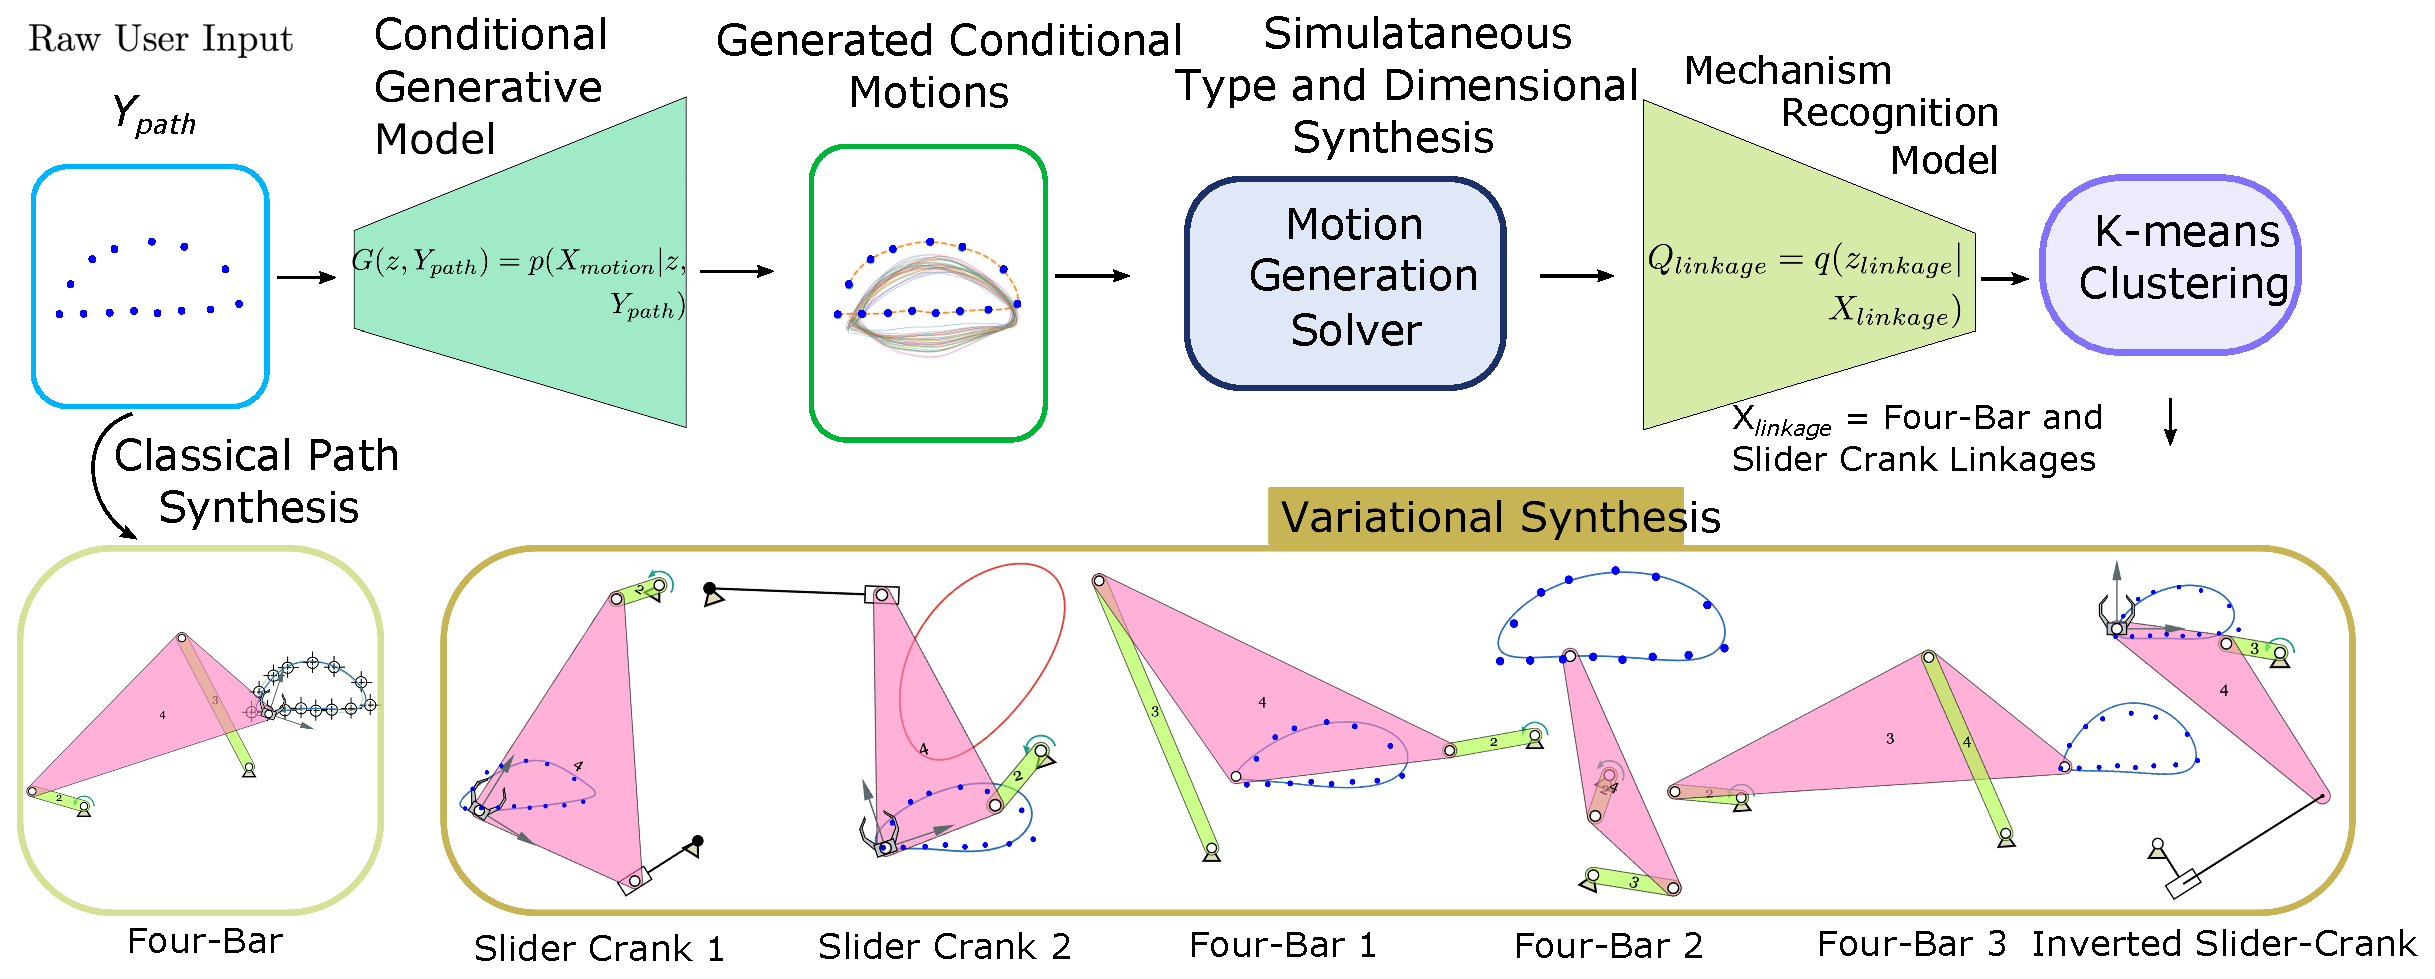
\includegraphics[width=\textwidth]{jmd-19/figure/fig_user_interaction_2.eps}
  \caption{C-VAE generates coupler motions corresponding to the path input. The orientation information of generated motion is not shown for cleaner illustrations. The generated motions are fed as inputs for the motion generation problem. The solutions solved by \cite{generalfitting-JCISE} are passed through a linkage recognition model which results predicts the latent distribution for each solution. This mixture of distributions is clustered to form distinctive concept distributions. The four-bar linkage in the bottom left corner depicts the optimal path synthesis solution using~\cite{sharma2019optimal}.}
\label{fig_user_interaction}
\end{figure*}



\section{Feasibility Conditioning and Input Feedback on Image-based Task}\label{sec_task_conditioning_image}
Raw user input is defined as an image with a different distribution of pixel intensities than the ones the VAE has learned while training. 
If such an input image is fed to VAE, the recognition network tries to find the learned patterns in the input. The patterns with high correlation with learned patterns will receive a high score that will be passed through max-pooling layers and eventually reflect in the obtained latent distribution. If samples from that distribution are passed through the generative model, it will produce coupler curve-like images that share similar spatial attributes.
Figure~\ref{fig_prob_shift_effect} shows examples where VAE takes in raw inputs and computes feasible inputs that are used for downstream tasks for path generation. It can be seen that VAE shifts the probability assignments on the pixels of the raw input. Figure~\ref{fig_prob_shift_effect} highlights this effect on various raw inputs. This is used to provide feedback on the user input.    
Figure~\ref{fig_two_inputs} depicts the outcome of VAE construction for two different inputs. The input shown on the top can be closely approximated by a four-bar mechanism, whereas the other input is highly unlikely for a four-bar or six-bar to interpolate. Since the VAE is trained on coupler curves of four-bar and six-bar linkages, it can reconstruct the original input with high accuracy. On the other hand, second input is highly modified by VAE to change it into a more conducive input. The difference between the modification done by VAE is reflected in the percentage change in the histogram of pixel intensities. For the first image, almost $70\%$ of the pixels retain their original $100\%$ intensity, whereas that number is a mere $17\%$ for the second input. 

\begin{figure*}
\centering
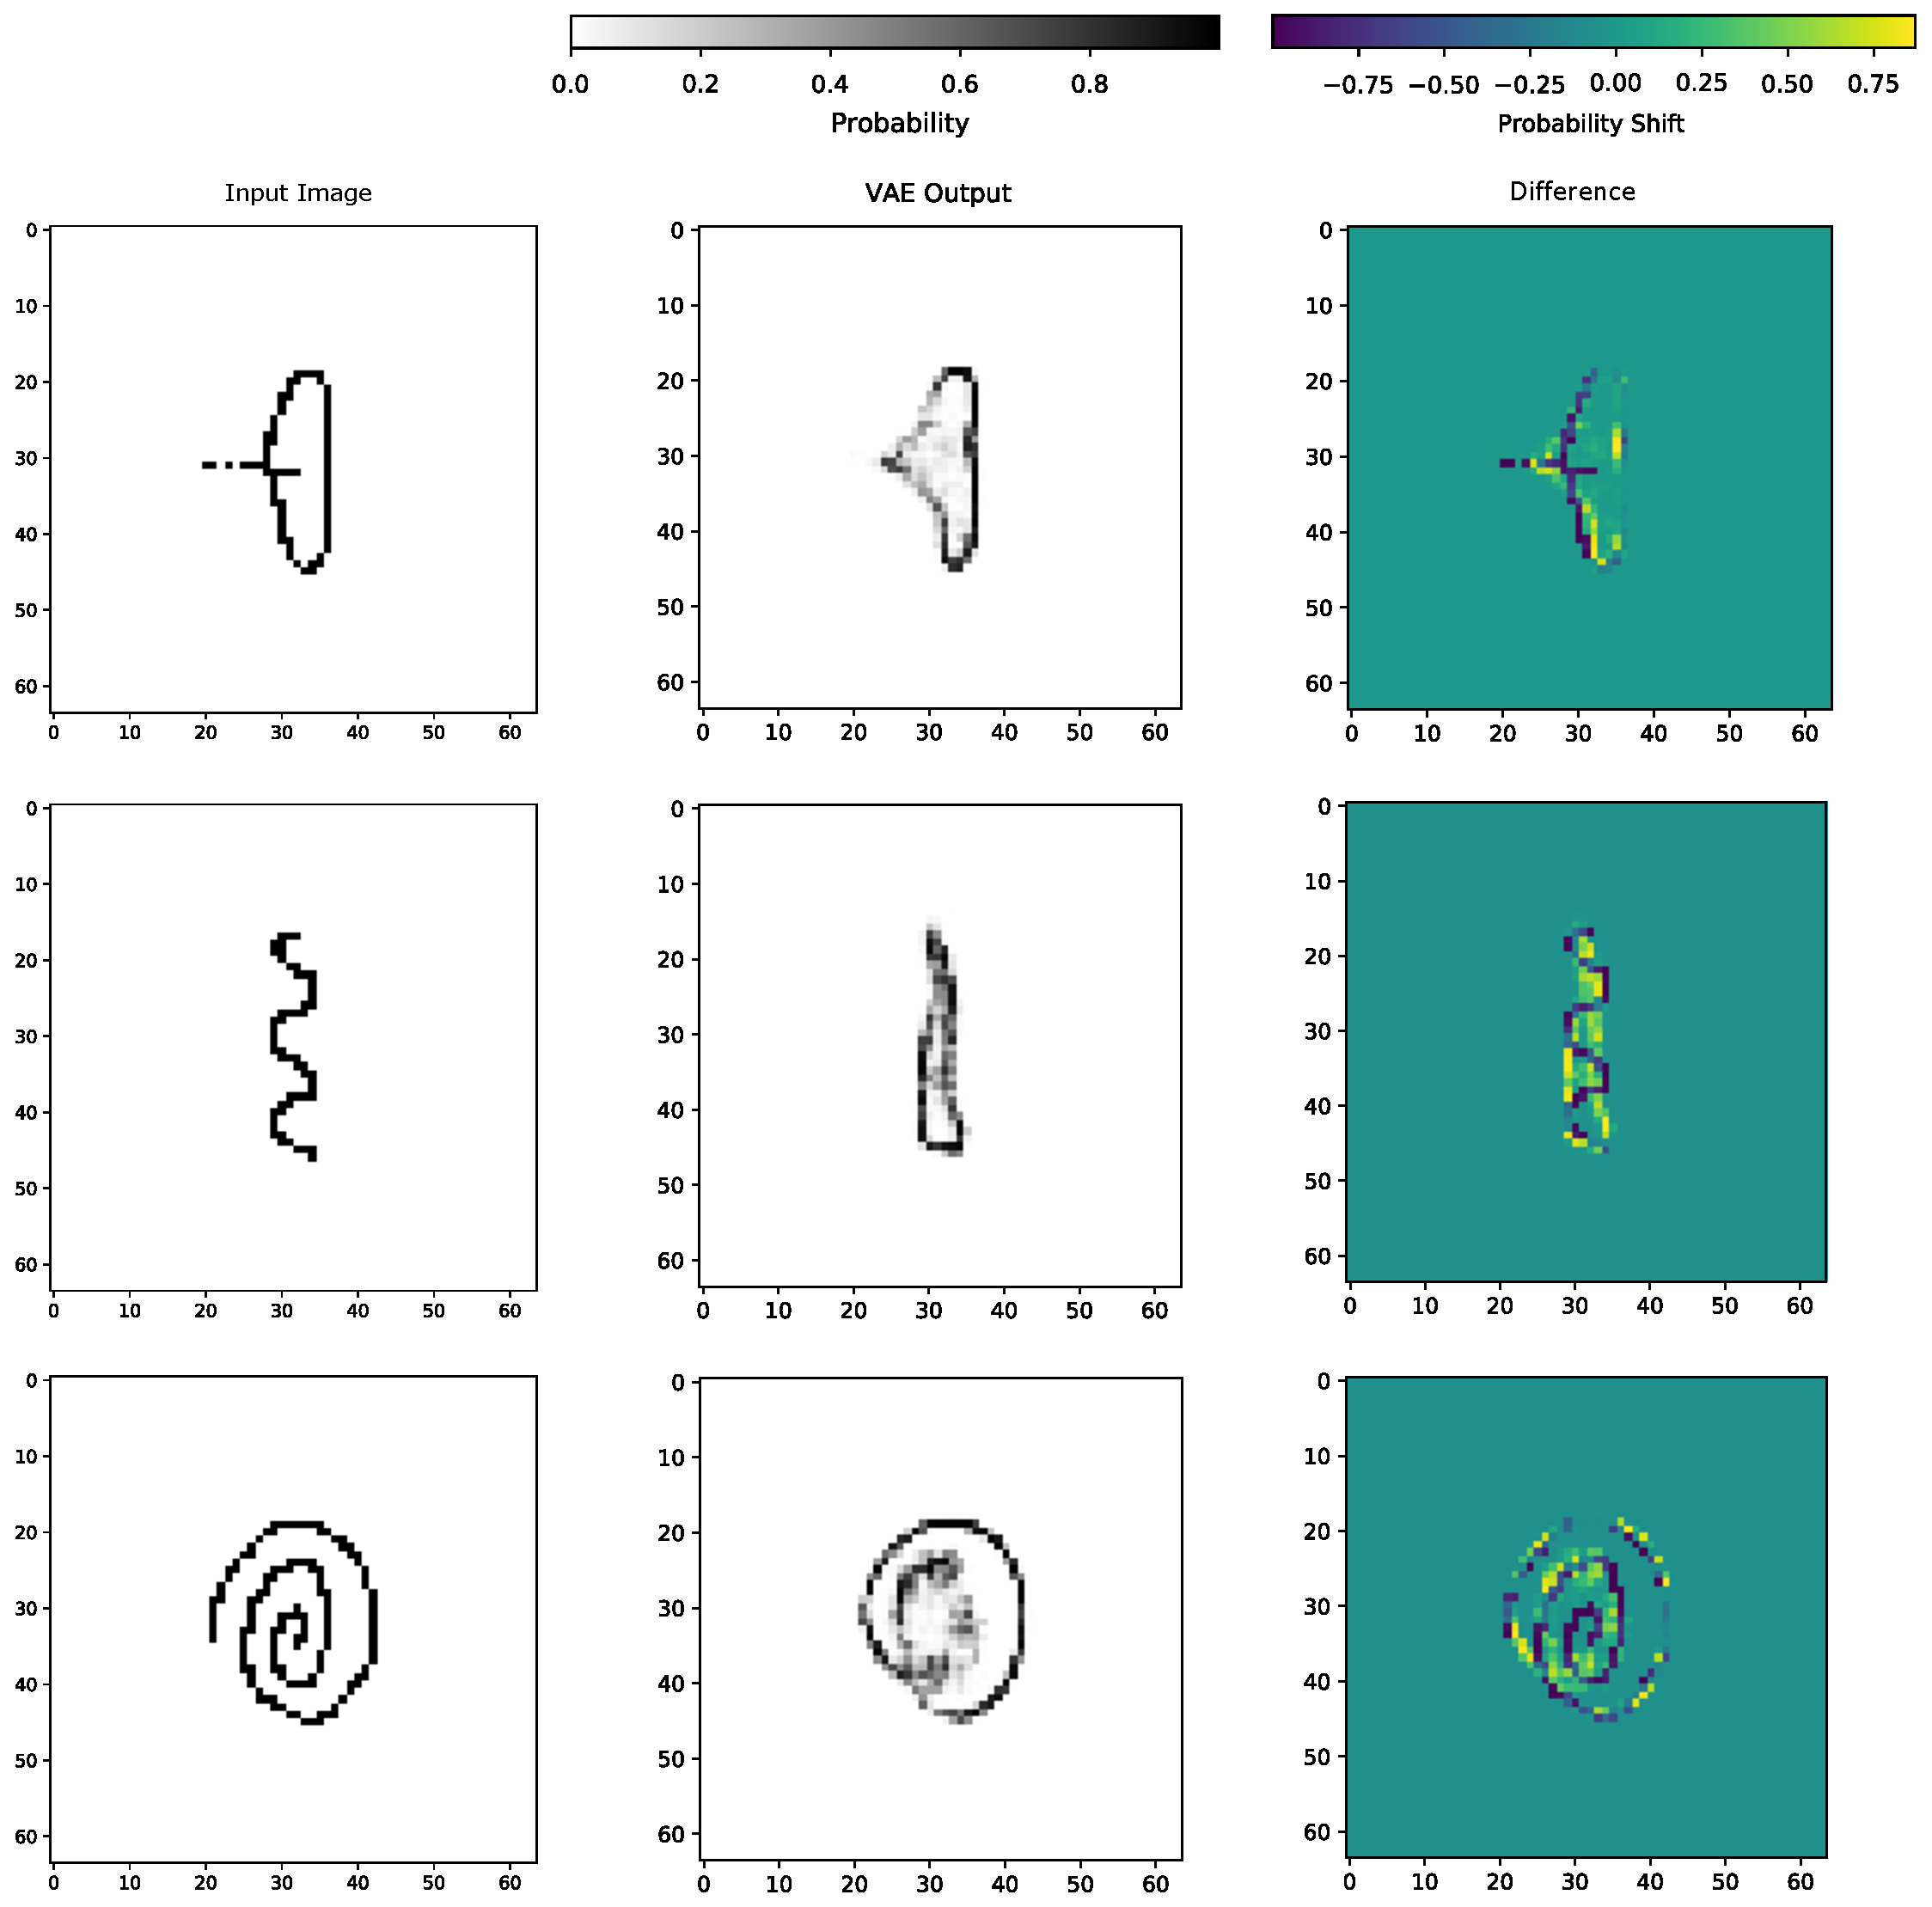
\includegraphics[width=0.75\textwidth]{idetc-20/figure/probability_shift.eps}
  \caption{Raw input image is passed through VAE which provides a feasible input image. The shift in the probabilities is highlighted in the rightmost images. The shift shown in dark indicates that the portion of raw input is highly unlikely for linkage from the dataset to interpolate. This provides visual and intuitive feedback to the user on the input.}
\label{fig_prob_shift_effect}
\end{figure*}

\begin{figure*}
\centering
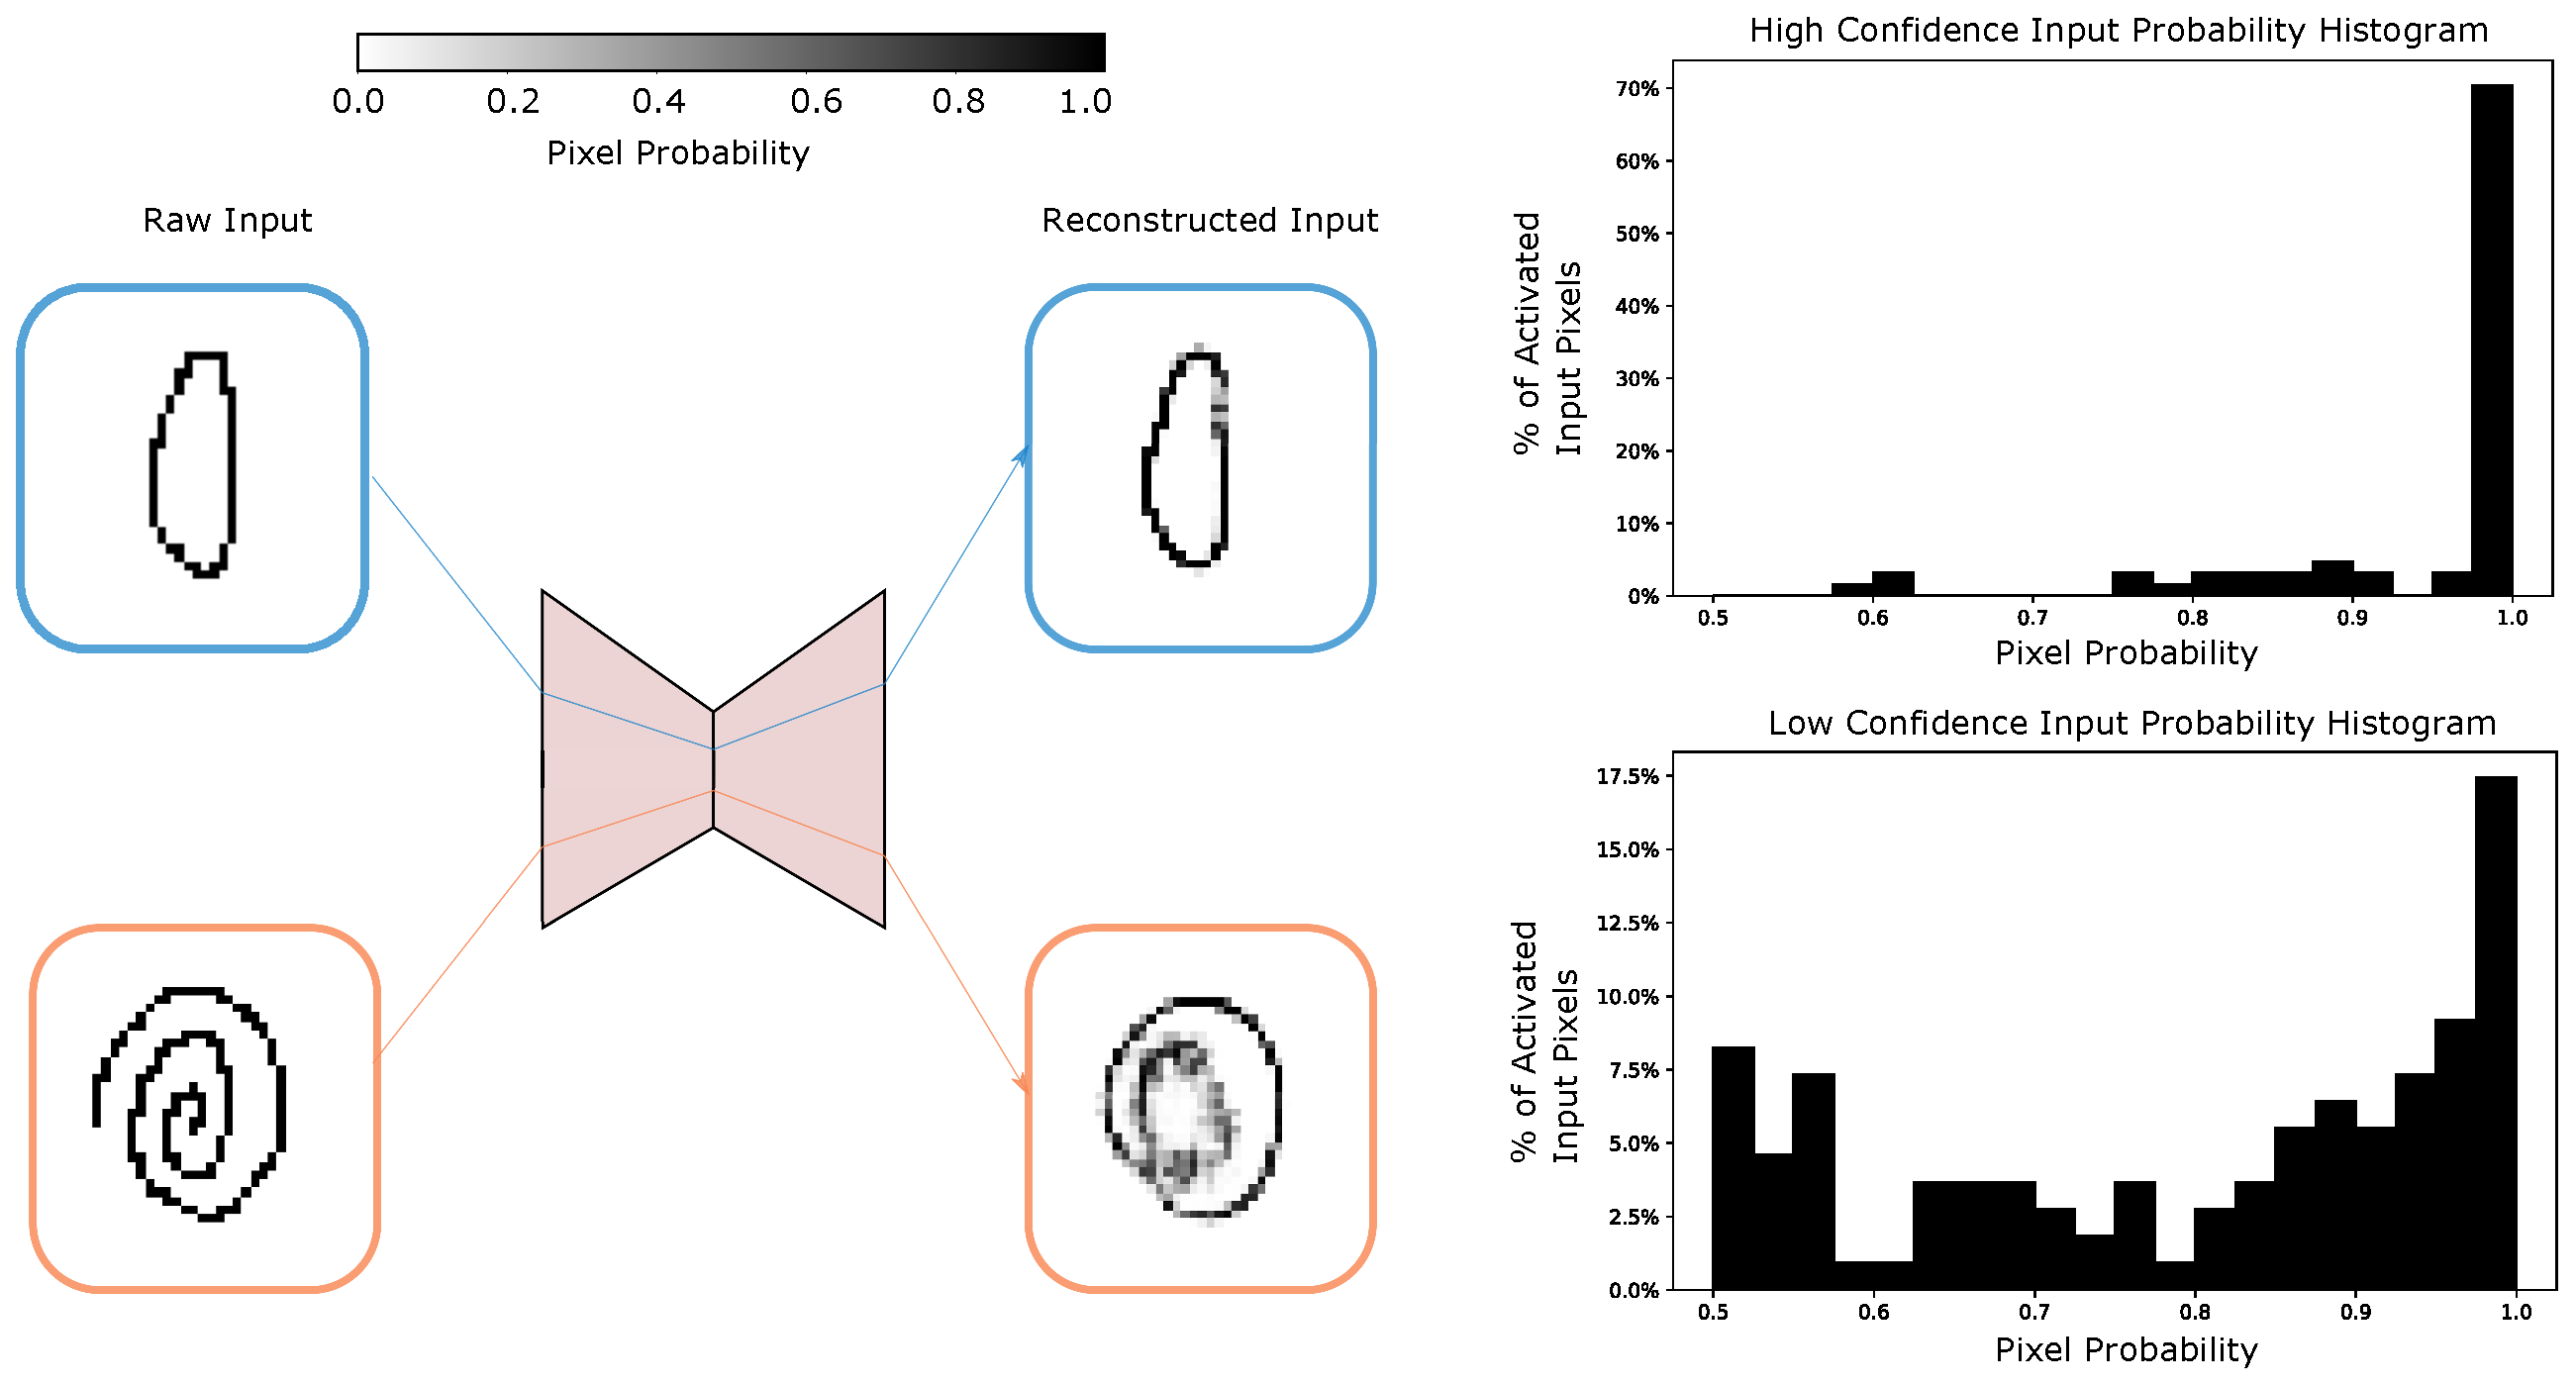
\includegraphics[width=\textwidth]{idetc-20/figure/high_low_confidence_feedback_new.eps}
  \caption{The raw input on the top is close to the true distribution of coupler curves, thus VAE retains almost $70\%$ of the highest intensities as depicted by the histogram on the top. For the second input, VAE overrides user assignments on the input pixels by a large number. This is due to the highly spiral nature of the input. It can be also seen in Fig~\ref{fig_prob_shift_effect} that the inner portion of the input is highly penalized. }
\label{fig_two_inputs}
\end{figure*}


\section{Latent Space Exploration}
During training, VAE learns to encode \ac{X} in a prior distribution which in our case is a multivariate Gaussian. Latent vector $z$ corresponding to \ac{X} is distributed such that the reconstructions $G(z)$ share similar spatial features. Figure~\ref{fig_latent_space_interactions} presents an example where a known coupler image \ac{x_path_im} is passed through recognition model of VAE with ten-dimensional latent space to obtain its mean latent embedding $z_{\mu}$. Then the latent embedding is shifted along each axisymmetric direction and the corresponding latent vector is reconstructed via generative model. It can be seen in Fig.~\ref{fig_latent_space_interactions} that the neighboring reconstructions not only share similar spatial features they smoothly morph into other feasible coupler images. This property can be exploited to make higher-level changes to \ac{x_task}.

\begin{figure*}
\centering
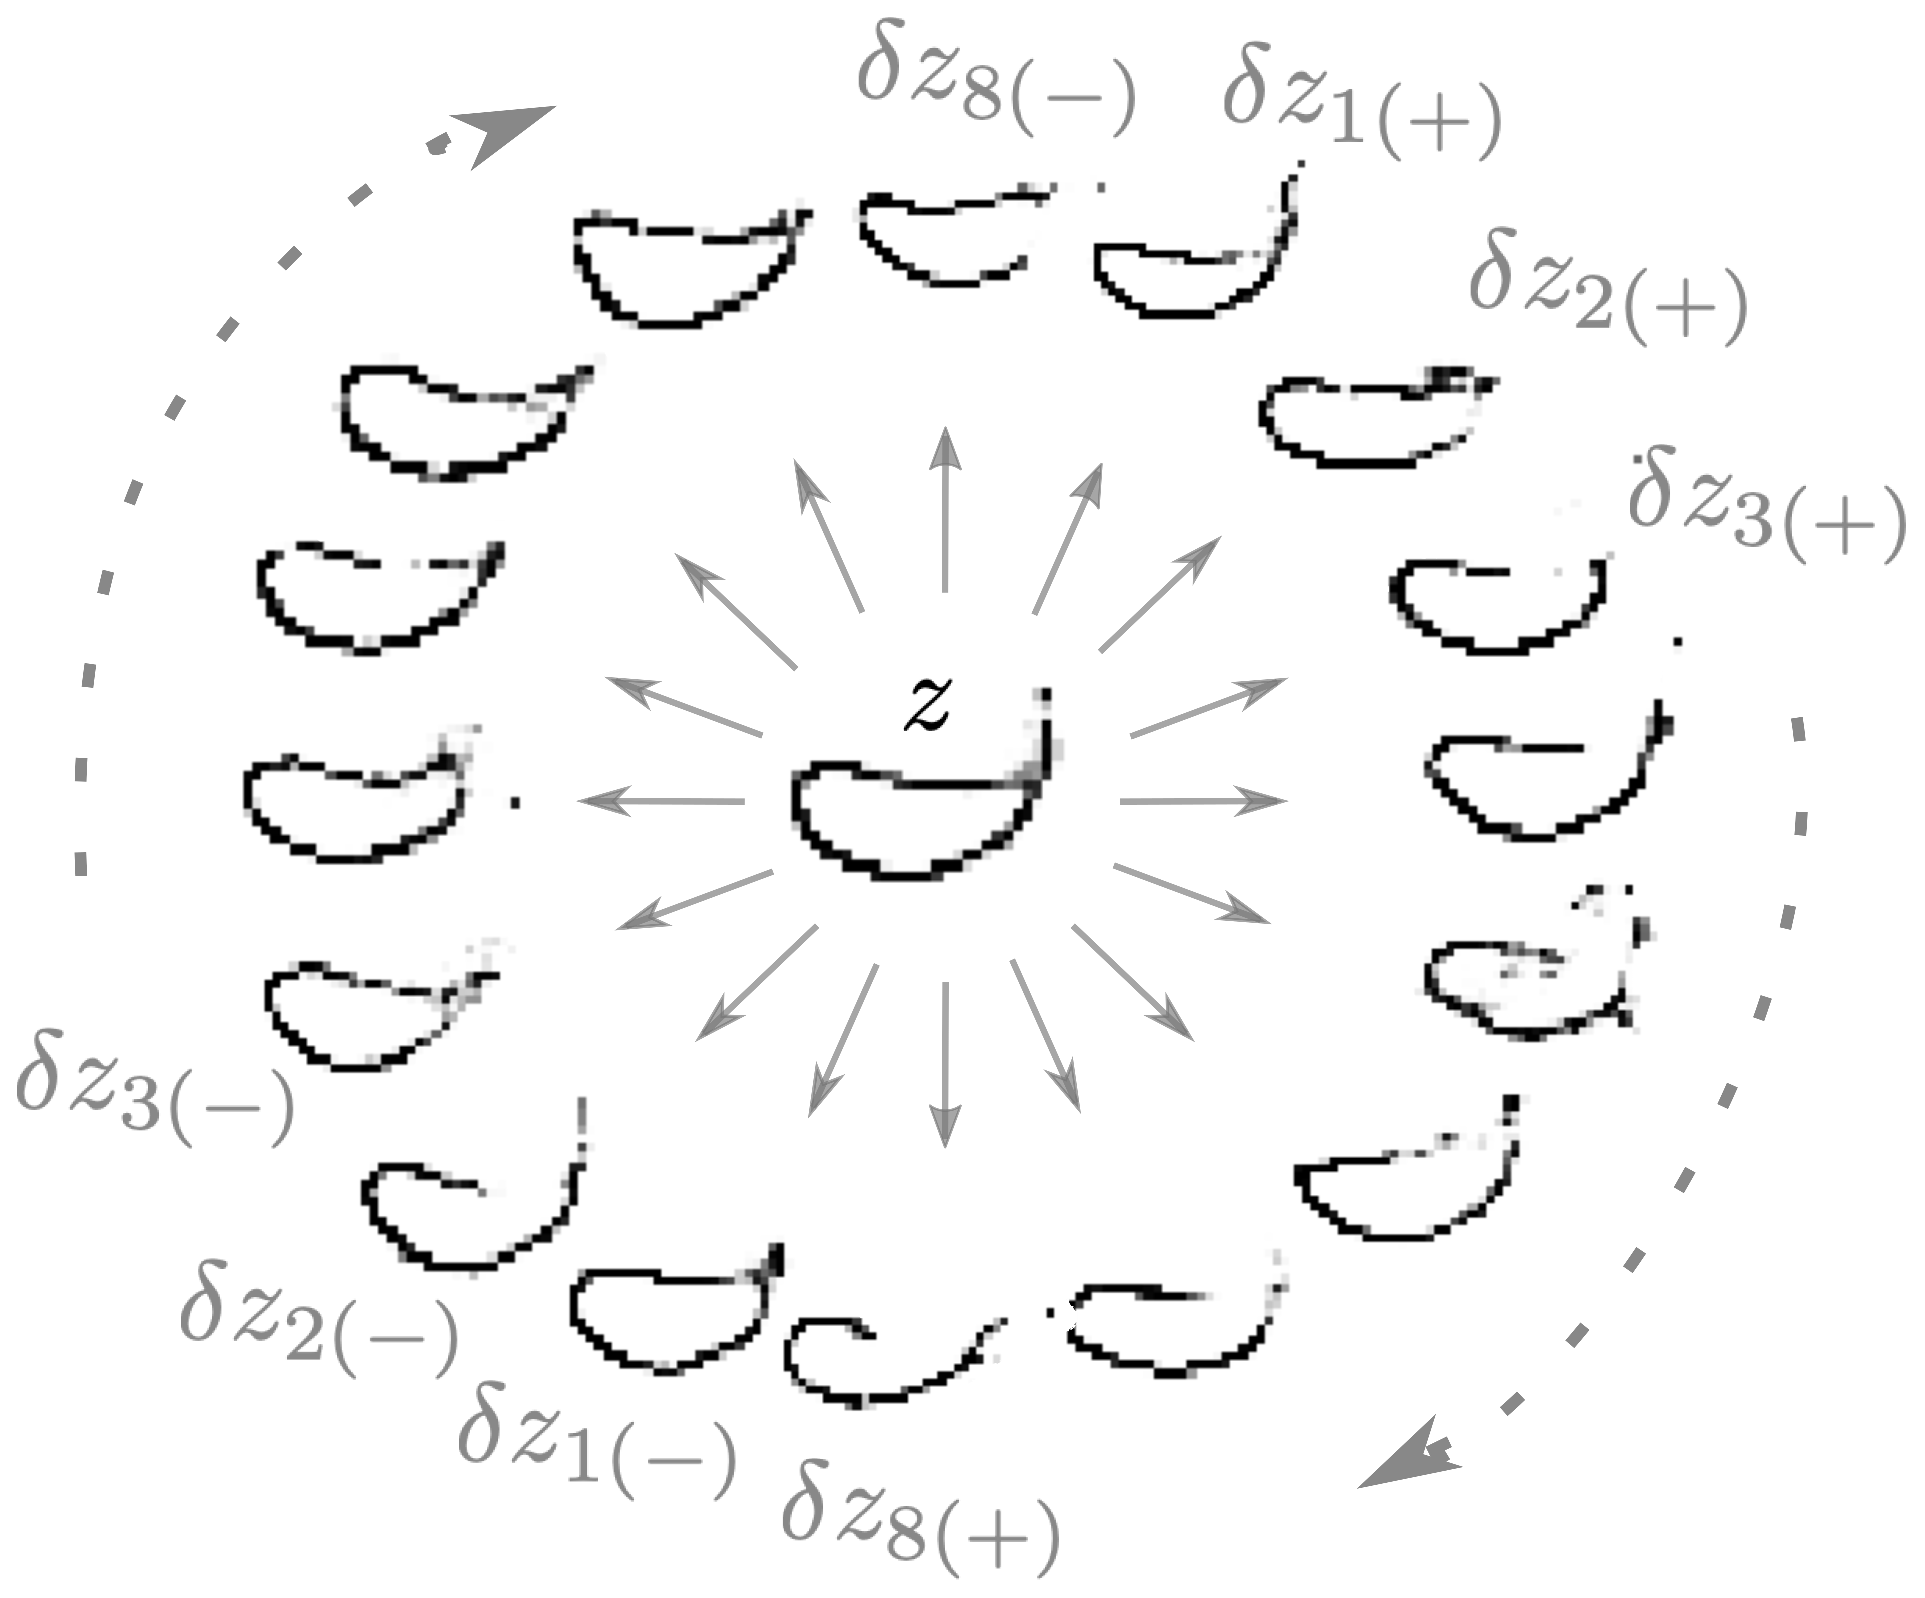
\includegraphics[width=0.55\textwidth]{idetc-20/figure/fig_latent_exploration.eps}
  \caption{Latent exploration in axisymmetric directions is depicted. The original latent vector $z$ is translated in axisymmetric directions. The arrow towards $\delta z_{1(+}$ indicates $z$ is translated in positive direction along $z1$ axis in ten-dimensional space.}
\label{fig_latent_space_interactions}
\end{figure*}

\subsection{Informed Latent Exploration}
Latent space allows us to navigate on a manifold of feasible coupler curve images. We can further exploit this by performing an informed exploration. Let us consider an example where the objective is to design a re-configurable linkage that satisfies a family of coupler curves. This family of coupler curves can be represented by a curve in latent space. VAE can be used to find a family of curves that morph from one curve to another by interpolation between the two latent curves. Figure ~\ref{fig_latent_space_interpolations} show a few examples of such interpolations.  
Although it should be noted that not all possible curves in latent space may correspond to feasible families of coupler curves. This is due to the possibility that the latent space may contain some void spaces as depicted by Fig~\ref{fig_latent_space_gaps}. This happens if certain data samples are drastically different from others.

\begin{figure}
\centering
\begin{tabular}{c}
1)\putindeepbox[7pt]{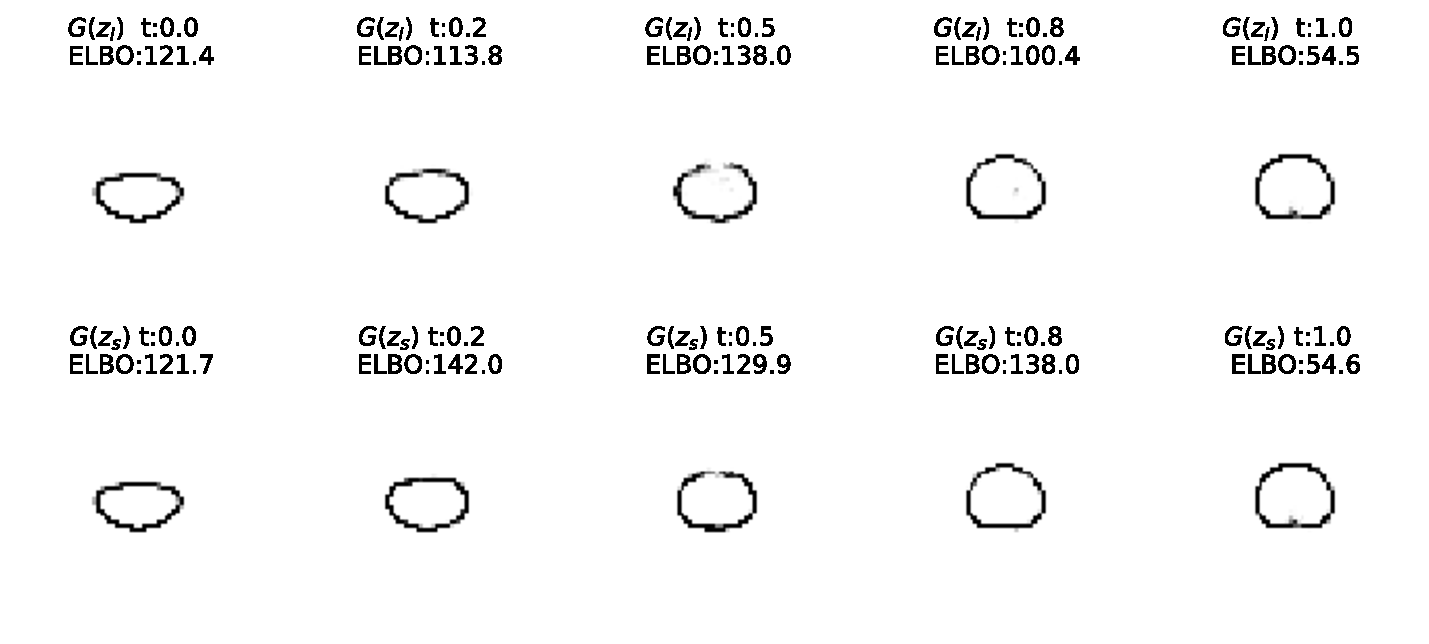
\includegraphics[width=0.95\textwidth]{idetc-20/figure/output_4_5.eps}}
  \\
2)\putindeepbox[7pt]{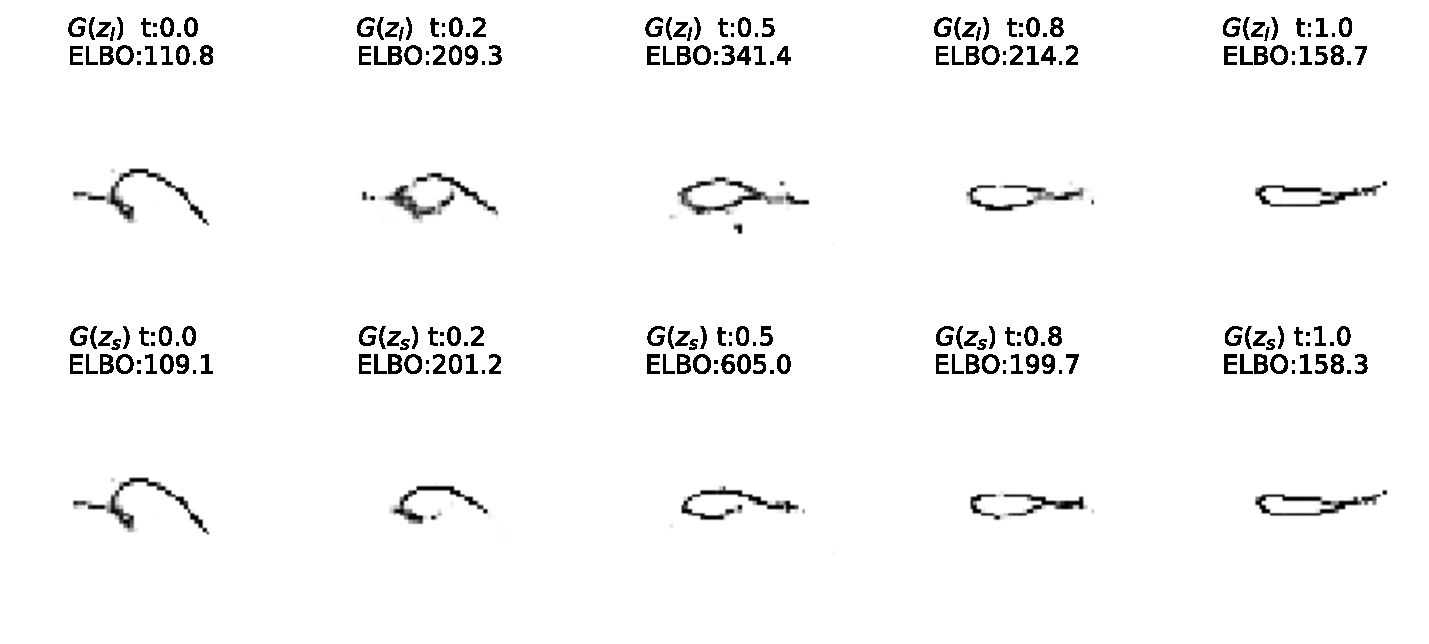
\includegraphics[width=0.95\textwidth]{idetc-20/figure/output_4_2.eps}} \\
3)\putindeepbox[7pt]{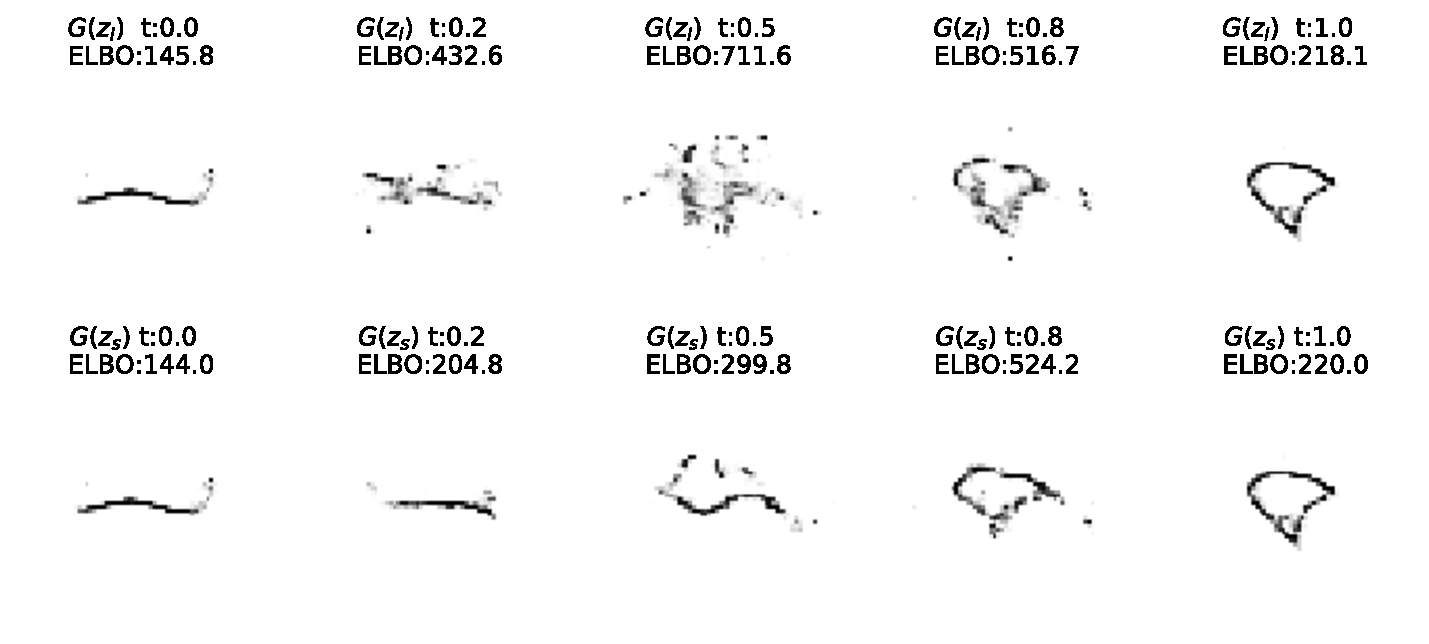
\includegraphics[width=0.95\textwidth]{idetc-20/figure/output_4_10.eps}}
\end{tabular}
\caption{Examples of linear and spherical interpolation between a pair of known coupler images. $G(z_l))$ and $G(z_s))$ denote reconstructions for linear and spherical interpolations respectively. It can seen that in some cases, the interpolation passes through infeasible region indicated by higher \ac{elbo_loss}.}
\label{fig_latent_space_interpolations}
\end{figure}

\begin{figure*}
\centering
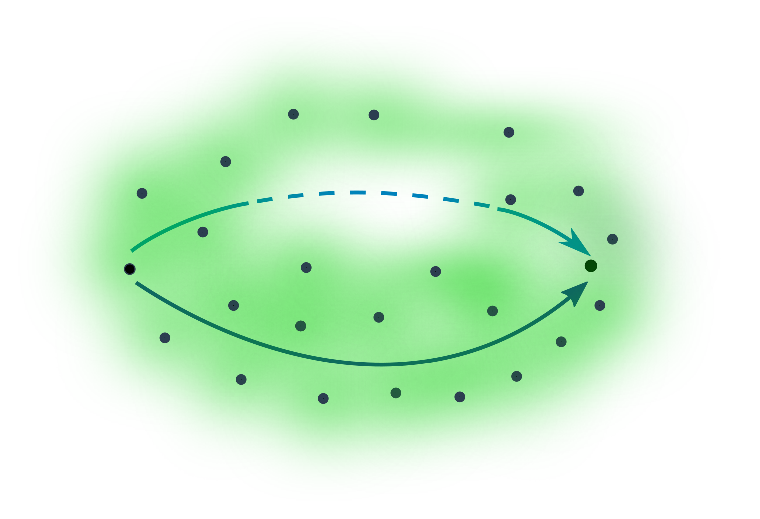
\includegraphics[width=0.45\textwidth]{idetc-20/figure/fig_latent_gaps.eps}
  \caption{Illustration of gaps in latent spaces that lead to higher reconstruction errors if a sample is drawn from those regions. Two interpolation strategies are shown, one of which passes through the infeasible region.}
\label{fig_latent_space_gaps}
\end{figure*}



\section{Context Conditioning}\label{sec_context}
Until now, we have seen that the latent space $z$ of a \ac{vae} trained on real data $X$ can be used to reconstruct samples $\hat{X}$ that have a high similarity to $X$. This section presents a strategy to explore the latent space in a more effectively to generate a samples \ac{x_hat_context} that maximize a fitness function \ac{context_function}. The algorithm for context conditioning is given in Algorithm~\ref{alg_context_conditioning},
\begin{algorithm}
    \SetKwInOut{Input}{Input}
    \SetKwInOut{Output}{Output}
    \Input{\ac{x_task}, $f(X) = $ \ac{context_function}} 
    \Output{\ac{x_hat_context}}
    $\mu, \sigma$ = \ac{q_x_task}(Input); \Comment{task recognition} \\
    $z_{\text{init}}$ = $\mathcal{N}(\mu, \sigma)$ \Comment{Initial starting point} \\
    $z$ = $z_{\text{init}}$ \\
    $\frac{\delta f(\hat{X})}{\delta z} = \frac{\delta f(\hat{X})}{\delta \hat{X}} \frac{\delta \hat{X}}{\delta z} = 
    \frac{\delta f(\hat{X})}{\delta \hat{X}} \frac{\delta G(z)}{\delta z}
    $ \Comment{$\frac{\delta f(\hat{X})}{\delta \hat{X}}$ and $\frac{\delta G(z)}{\delta z}$ are analytically known}  \\
    \textbf{Maximize f(X)} w.r.t. $z$ \Comment{Using Stochastic Backpropagation}\\
     using gradients $\frac{\delta f(\hat{X})}{\delta z}$\\
     Subject to, \\
     $||z_{new} - z_{init}|| < \text{Z}_{\text{Threshold}}$,\\
     $\mathcal{L}_{\text{ELBO}}(G(z)) <  \text{ELBO}_{\text{Threshold}}$ \Comment{ Suitable thresholds should be chosen }\\
     \textbf{return} $G(z)$
    \caption{Contextual Latent Exploration}
    \label{alg_context_conditioning}
\end{algorithm}

It can be argued that if there exist a continuous function \ac{context_function} then one can simple perform the search of $X$ that maximizes \ac{context_function}. However, the distribution of real $X$ data is non-continuous and occupies a much smaller dimension in its high dimensional domain. Thus, a direct optimization w.r.t. $X$ can get lost into large infeasible regions of $X$. In addition, searching in ow dimensional $z$ space is more efficient and the results are more semantically similar $X$ to the original task \ac{x_task}. It should be noted that the objective is not to cause significant changes to the original task \ac{x_task}.  

\subsection{Context as Desired Fixed Pivot Regions}
In the case of one degree-of-freedom linkages, there exists a definite relationship between fixed pivots and the coupler curve of the linkage. In the case of four-bar linkage, three linkages exist that can trace the exact same curve. The set of such linkages are called cognates. The number of cognates can be different for different topologies.

In this case, we use the data-driven approach to learn the relationship between coupler curves and the corresponding fixed pivot locations by training a neural network. Instead of training a regression model that predicts the exact fixed pivot locations, we train a set of classifier models that predicts the probability of a discretized region containing a fixed pivot. This is shown in Fig.~\ref{fig_fix_pivot_discretization}.

\begin{figure*}
\centering
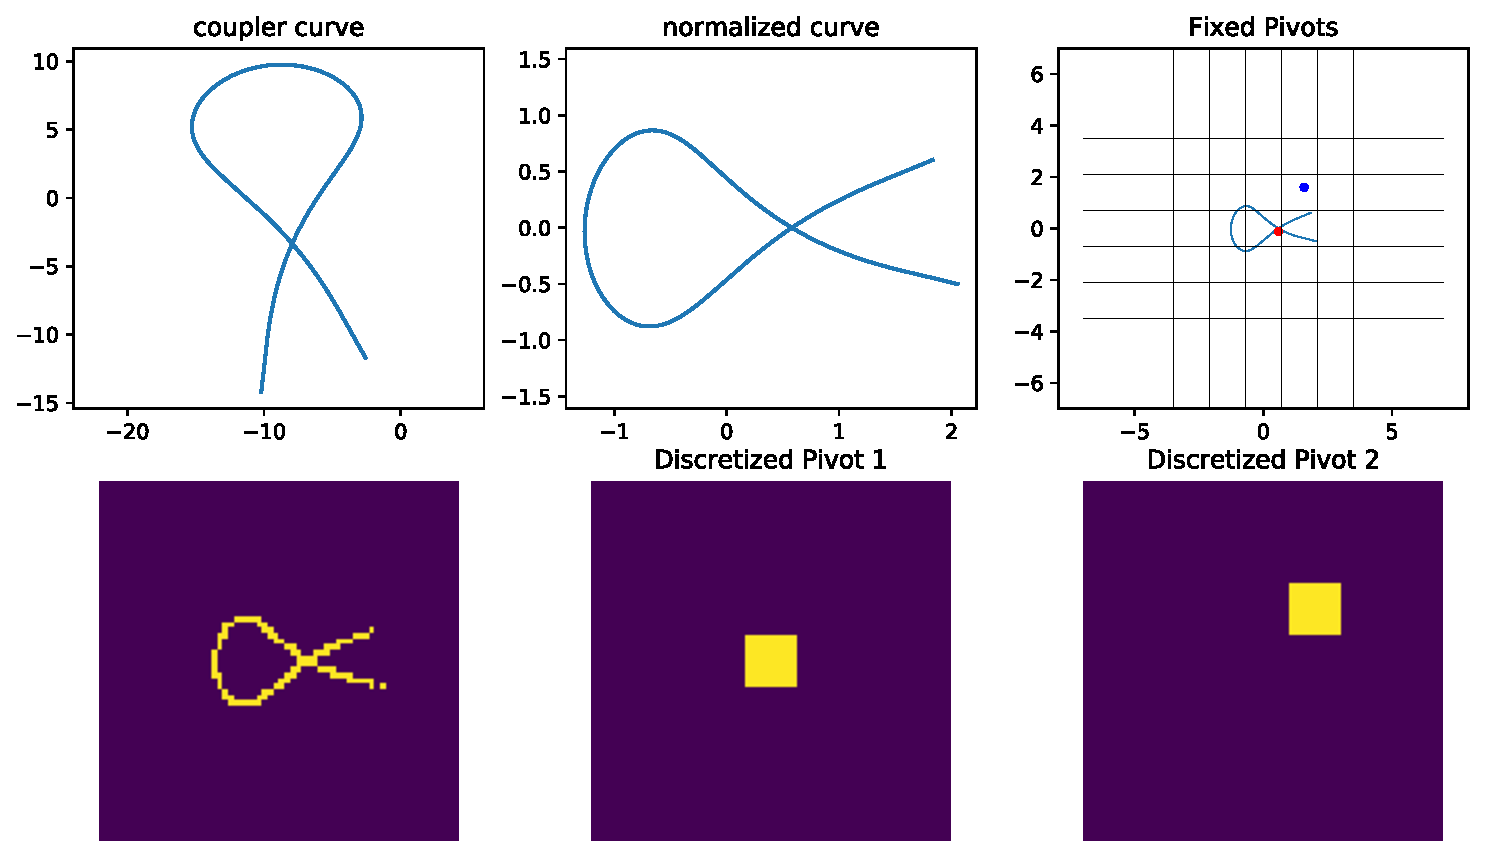
\includegraphics[width=0.95\textwidth]{idetc-20/figure/fig_fix_pivot_discretization.eps}
  \caption{The fixed pivots for the linkage are transformed according to the normalization of the coupler curve. The location of each fixed pivot is discretized to create a one-hot vector of 49 dimensions, depicted in an image form.}
\label{fig_fix_pivot_discretization}
\end{figure*}

The 2D space for fixed pivot prediction is discretized into $k\times k$ pixels, where $k$ is the number of divisions along $x$ or $y$ axis. Here we take $k = 7$. 
The objective for classifier ($FP$) is to learn a set of functions ${FP_{i,j}(X_{64\times 64})}_{i=1, j=1}^{i=7, j=7}$, where each function $FP_{i,j}$ predicts the probability of the region covered by pixel at ${i,j}$.
Since one coupler curve can be traced by many linkages (three for four-bar), $FP(X)$ should predict multiple possibilities in terms of a probability distribution.

For $i=7, j=7$, $f$ comprises of total 49 functions. For the input $X$ shown above, it should predict at least two possibilities. The below figure displays the expected output for $X$. A classifier is trained that predicts a probability for each of the $49$ pixels.
Figure~\ref{fig_classifier_output} presents classification result of a sample input. 

\begin{figure*}
\centering
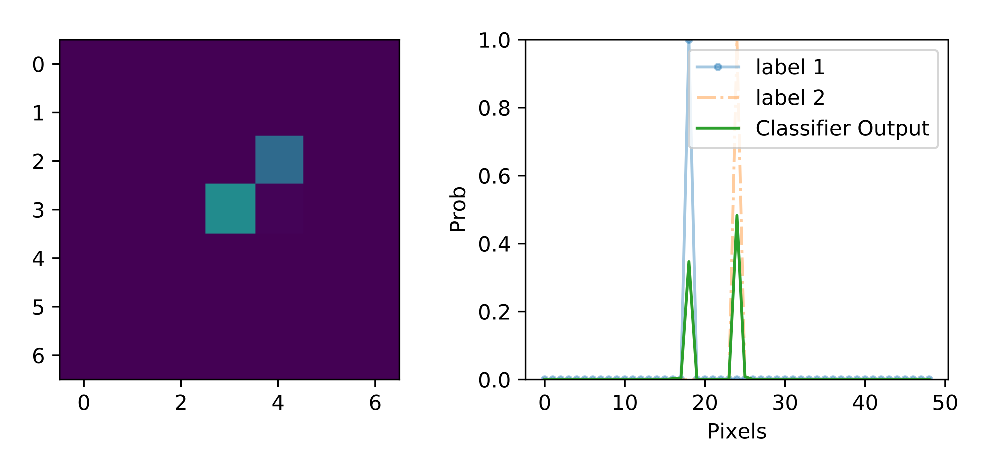
\includegraphics[width=0.95\textwidth]{idetc-20/figure/fig_classifier_output.eps}
  \caption{Classifier predicts a probability for each of the 49 pixels. The probability indicates the likelihood that the region spanned by that pixel contains a fixed pivot. The pixels where the fixed pivot lie are given a significantly high probability than the rest of the pixels.}
\label{fig_classifier_output}
\end{figure*}

\begin{figure*}
\centering
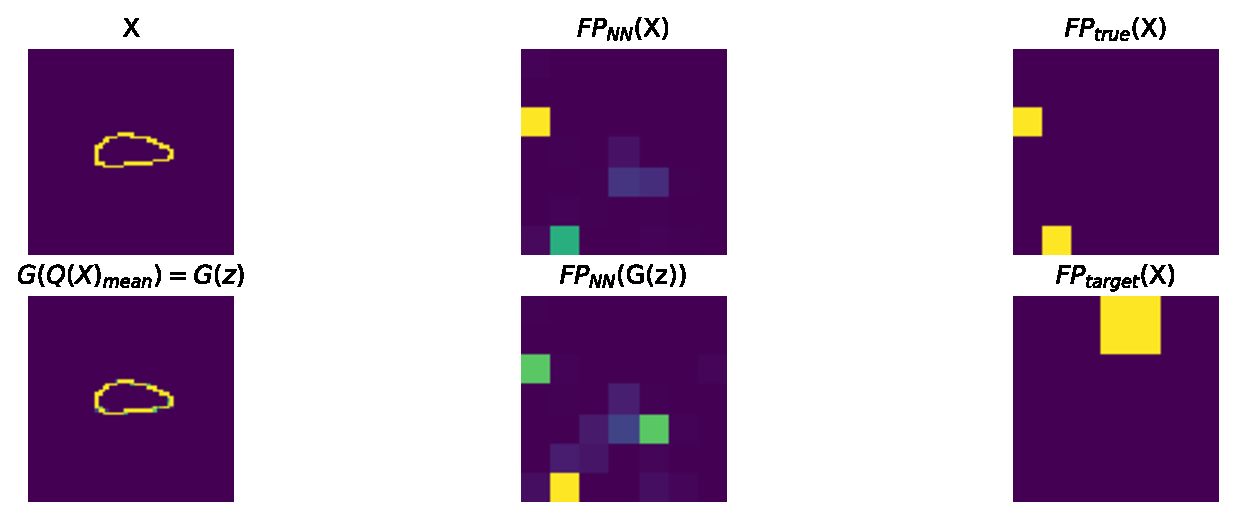
\includegraphics[width=0.95\textwidth]{idetc-20/figure/fig_x_input_for_context_conditioning.eps}
  \caption{The approach start with a linkage with coupler curve image $X$ and fixed pivots at $FP_{true}(X)$. A trained classifier $FP_{NN}(X)$ accurately predicts the true location of fixed pivots. The $X$ is reconstructed using a trained generative model which will be used in context conditioning. The image titled $FP_{target}(X)$ highlights a portion of classifier which will be subjected to maximization in the optimization routine given in Algorithm~\ref{alg_context_conditioning}.}
\label{fig_x_input_for_context_conditioning}
\end{figure*}


\begin{figure*}
\centering
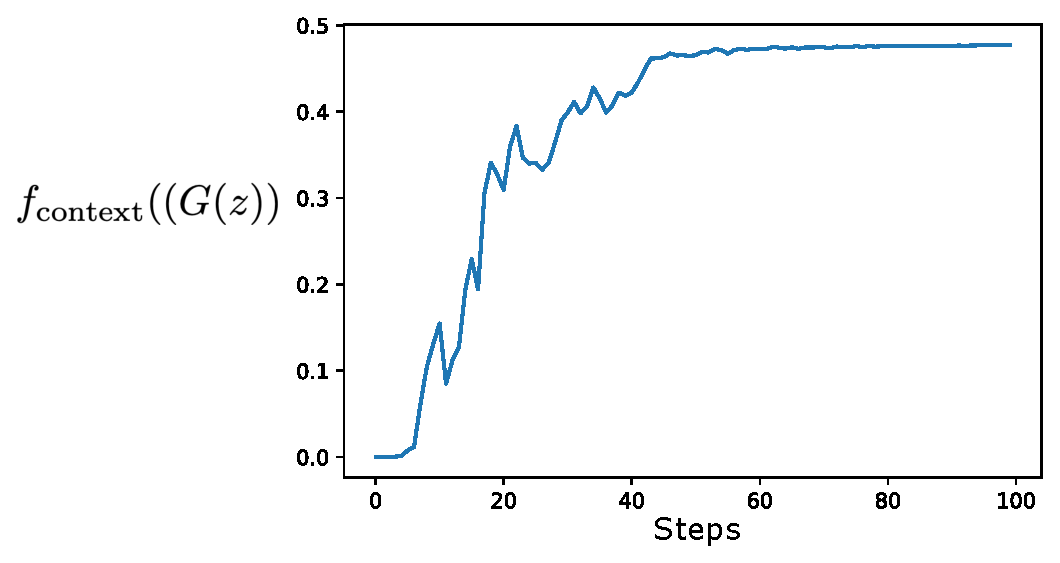
\includegraphics[width=0.65\textwidth]{idetc-20/figure/fig_context_optimization_graph.eps}
  \caption{Value of objective function over 100 steps of gradient based stochastic optimization.}
\label{fig_context_optimization_graph}
\end{figure*}

\begin{figure*}
\centering
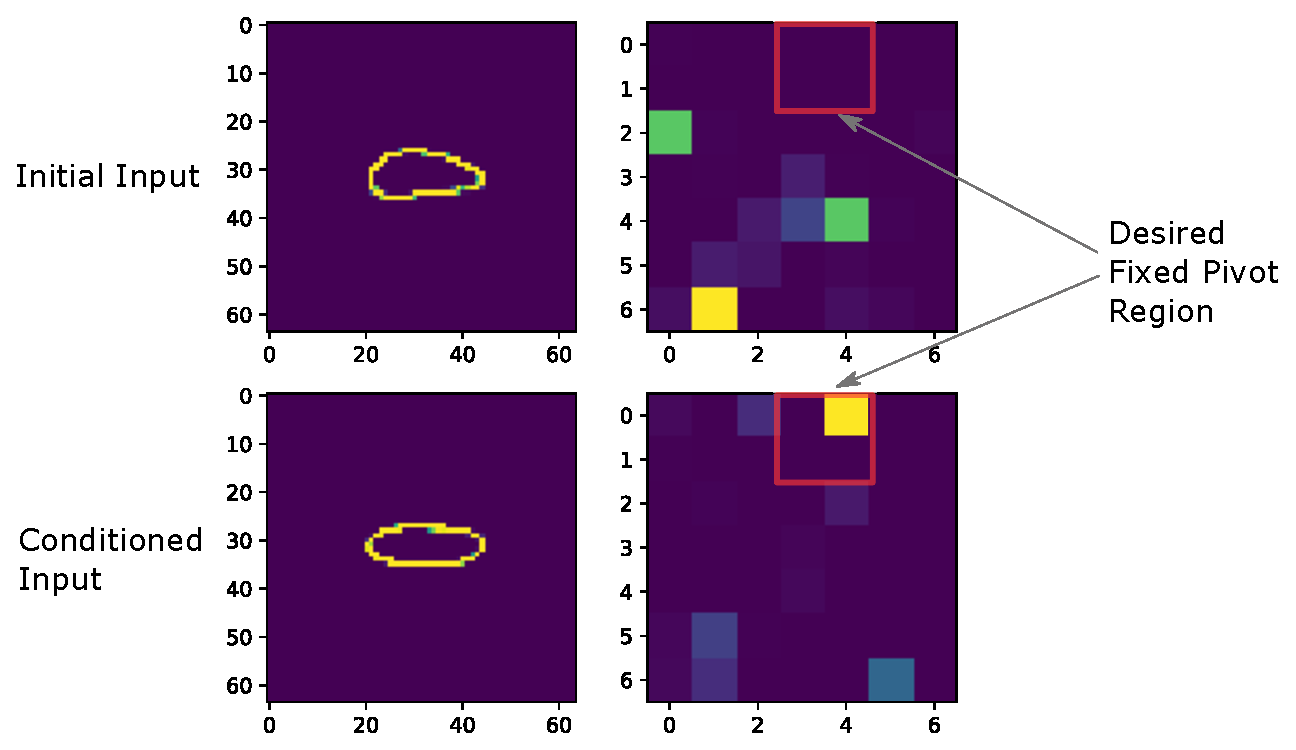
\includegraphics[width=0.95\textwidth]{idetc-20/figure/fig_context_conditioning_result.eps}
  \caption{Initial and final coupler curve images with their corresponding fixed pivot region predictions. It can be seen that only subtle changes in the coupler curve are needed to satisfy the desired fixed pivot predictions.}
\label{fig_context_conditioning_result}
\end{figure*}

We use this classifier as the context function to make small informed changes in a task image depicted in Fig.~\ref{fig_x_input_for_context_conditioning}. $FP_{target}(X)$ in Fig.~\ref{fig_x_input_for_context_conditioning} depicts a binary mask. This mask is multiplied with the output of the classifier. Summation of the above product is treated as the fitness function in context conditioning given by,
\begin{equation}
    f_{\text{context}}(X) = \sum_{i=1, j=1}^{i=7, j=7} {FP(X)} \cdot FP_{\text{target}}(X)
\end{equation}


Then the procedure presented in Algorithm~\ref{alg_context_conditioning} is followed.
This procedure conducts an informed exploration in the latent space that maximizes the fitness function. Figure~\ref{fig_context_optimization_graph} depicts the increase in value of objective function as the optimization progress. Figure~\ref{fig_context_conditioning_result} depicts the initial and final coupler curve images. It can be seen that only subtle changes in the coupler curve are needed to satisfy the desired fixed pivot predictions. It should be noted that the output of context conditioning is not guaranteed to produce the solutions with fixed pivots lie in the desired region. However, it is an input that has a higher probability (indicated by trained classifier) of finding solutions with fixed pivots in the prescribed regions. In this work, we have developed a synthesis algorithm that provides theoretical guarantees to satisfy such practical constraints in the case of motion generation for four-bar linkage. The approach presented in this section, however, is more versatile and can incorporate any data-driven context and is invariant to linkage topology.    


\section{Nearest Latent Neighbors for Variational Path Synthesis}

In Section~\ref{sec_task_conditioning_image}, it was shown that the recognition network captures the spatial correlations that highly correspond to that of coupler curve images. To take advantage of this fact, the database is remapped into a 50-dimensional space where each mechanism is represented by the latent vector obtained using the recognition model. At the time of synthesis, raw input is passed through the recognition model to find a distribution of possible latent vectors. K-Nearest neighbors to the mean of this distribution are returned as potential solutions. Figure~\ref{fig_knn_latent} presents some of the solutions obtained for the nearest neighbor query on raw user input. 


\begin{figure*}
\centering
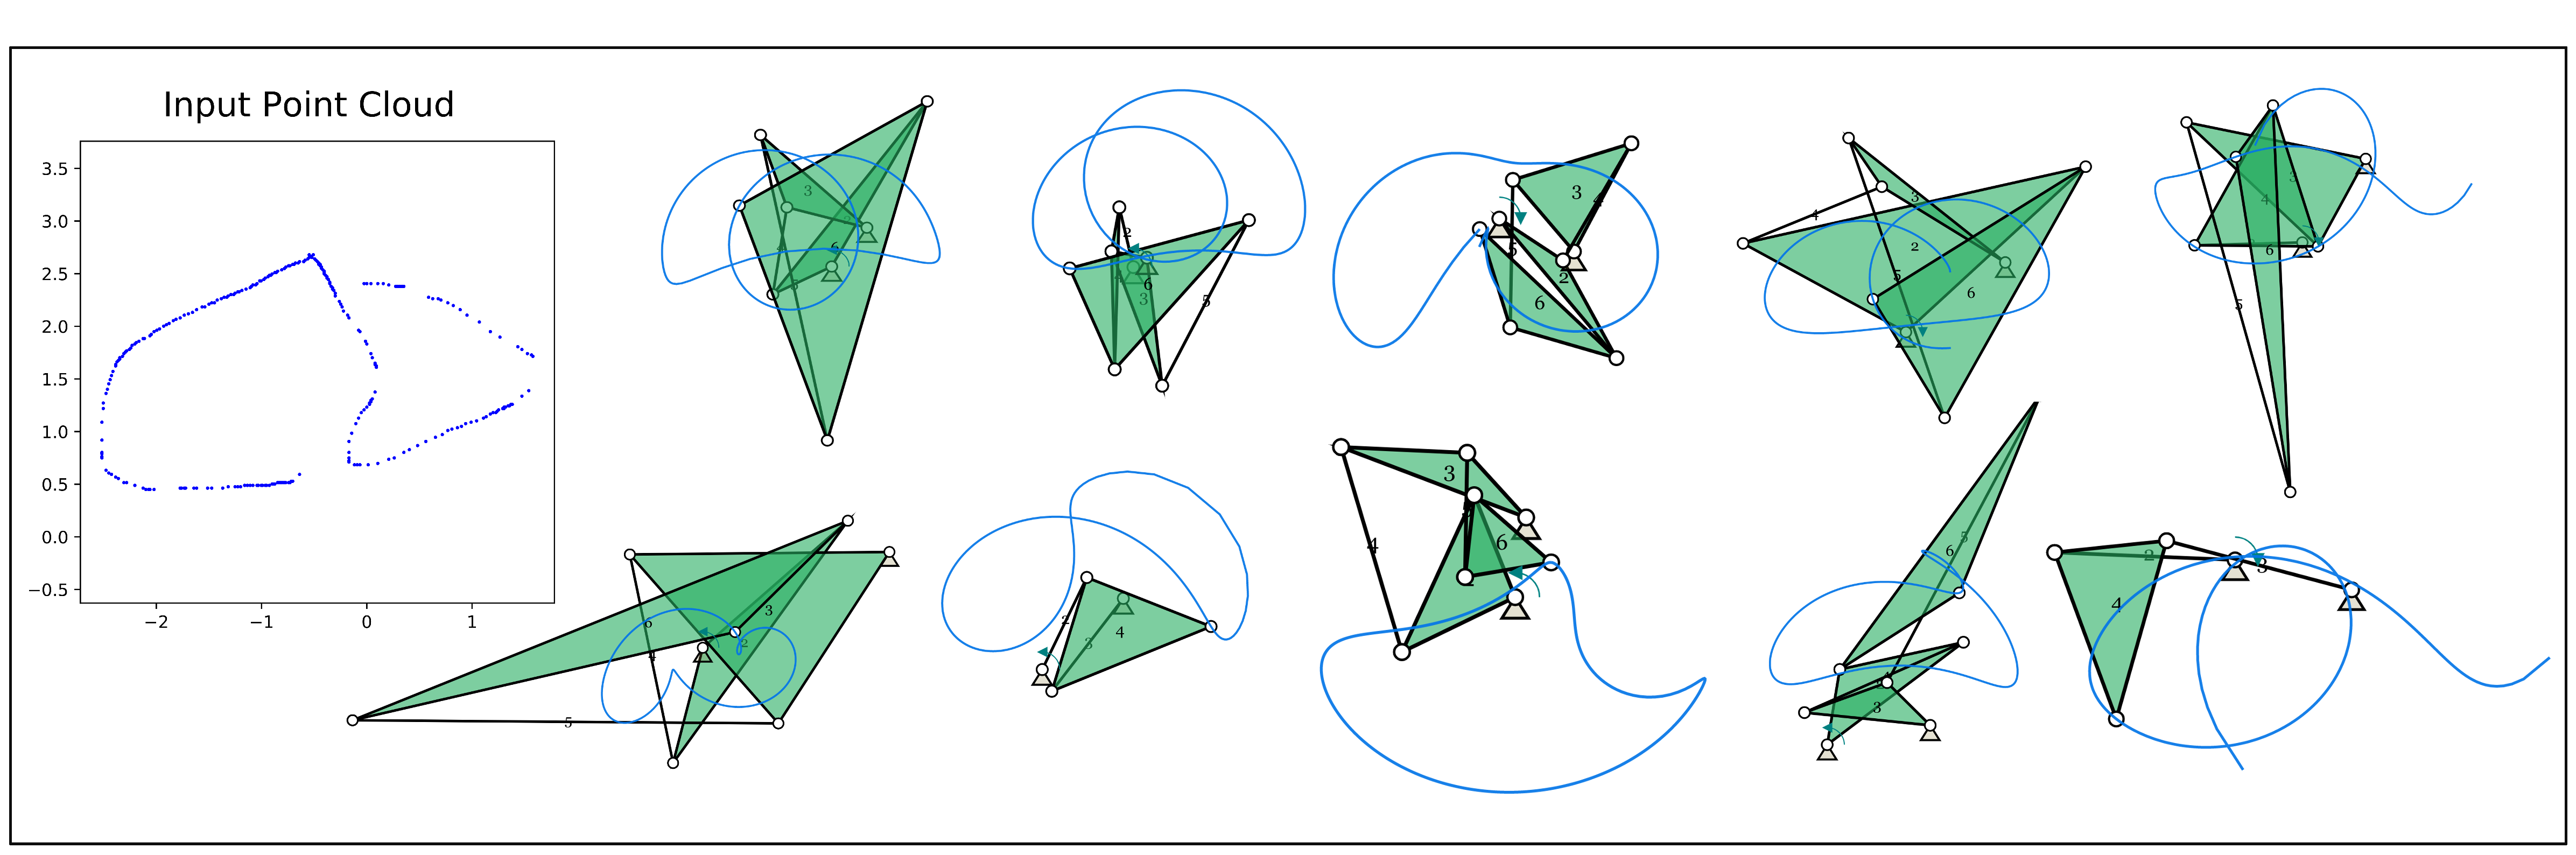
\includegraphics[width=0.85\textwidth]{idetc-20/figure/fig_knn_latent.eps}
  \caption{The linkages corresponding to the K nearest neighbor in latent space for the given raw input are depicted. It can be seen that the linkages exhibit a wide variety in terms of their coupler path; thereby capturing input uncertainty.}
\label{fig_knn_latent}
\end{figure*}

\section{Linkage Clustering}\label{subsec_vae_for_ln}
Consider a set of $M$ linkages represented by set of vectors, ${\{X_{linkage_{i}}\}}_{i=1}^{M}$.
Now, it is useful to find $K$ representative linkages that cover the variety of obtained solutions, where $K$ is a user-selected parameter.
To find such $K$ representative linkages, we perform K-means\cite{lloyd1982kmeans} Clustering on the set of $M$ linkages, where $K << M$.
Before performing clustering, we first pass the set through recognition module to obtain a compressed representation for the set $\{(\mu_{linkage_i}$, $\sigma_{linkage_i})\}_{i=1}^M$ given by,
\begin{equation}\label{eq_recogn_linkage}
  \mu_{linkage_i}, \sigma_{linkage_i} = Q_{linkage}(X_{linkage_i}; \theta_e).\\
\end{equation}
Where $Q_{linkage}$ is the recognition model of the VAE trained on the corresponding linkage dataset.

Now, for computing the pairwise distance between two linkages $X_{linkage_i}$ and $X_{linkage_j}$, we take the $L2$-norm between their corresponding mean latent vectors $\mu_i$ and $\mu_j$.
Using the $L2$-norm on latent representations instead of $L2$-norm on the original vectors has shown to yield better clustering for high dimensional data\cite{song2013}.
This results in the identification of $K$ clusters and along with the corresponding cluster centers.
Figure~\ref{fig_overview} shows cluster centers for the recognition and clustering task for a set of $100$ four-bar linkages with $K = 4$.
